\documentclass[12pt,oneside]{uhthesis}
\usepackage[noend]{algpseudocode}
\usepackage{fancyvrb}
\usepackage{hyperref}
\usepackage{subcaption}

% \usepackage{subfigure}
\usepackage[ruled,lined,linesnumbered,titlenumbered,algochapter,spanish,onelanguage]{algorithm2e}
\usepackage{amsmath}
\usepackage{amssymb}
\usepackage{amsbsy}
\usepackage{caption,booktabs}
\captionsetup{ justification = centering }
%\usepackage{mathpazo}
\usepackage{float}
\setlength{\marginparwidth}{2cm}
\usepackage{todonotes}
\usepackage{listings}
\usepackage{xcolor}
\usepackage{multicol}
\usepackage{graphicx}
\floatstyle{plaintop}
\restylefloat{table}
\addbibresource{Bibliography.bib}
% \setlength{\parskip}{\baselineskip}%
\renewcommand{\tablename}{Tabla}
\renewcommand{\listalgorithmcfname}{Índice de Algoritmos}
%\dontprintsemicolon
\SetAlgoNoEnd

\definecolor{codegreen}{rgb}{0,0.6,0}
\definecolor{codegray}{rgb}{0.5,0.5,0.5}
\definecolor{codepurple}{rgb}{0.58,0,0.82}
\definecolor{backcolour}{rgb}{0.95,0.95,0.92}

\lstdefinestyle{mystyle}{
    backgroundcolor=\color{backcolour},   
    commentstyle=\color{codegreen},
    keywordstyle=\color{purple},
    numberstyle=\tiny\color{codegray},
    stringstyle=\color{codepurple},
    basicstyle=\ttfamily\footnotesize,
    breakatwhitespace=false,         
    breaklines=true,                 
    captionpos=b,                    
    keepspaces=true,                 
    numbers=left,                    
    numbersep=5pt,                  
    showspaces=false,                
    showstringspaces=false,
    showtabs=false,                  
    tabsize=4
}

\lstset{style=mystyle}

\title{Gestión de Dominio}
\author{\\\vspace{0.25cm}Enmanuel Verdesia Suárez}
\advisor{\\\vspace{0.25cm}Lic. Alexi Massó Muñoz\\\vspace{0.2cm}Lic. Roberto Martí Cedeño}
\degree{Licenciado en Ciencia de la Computación}
\faculty{Facultad de Matemática y Computación}
\date{Fecha\\\vspace{0.25cm}\href{https://github.com/username/repo}{github.com/username/repo}}
\logo{Graphics/uhlogo}
\makenomenclature

\renewcommand{\vec}[1]{\boldsymbol{#1}}
\newcommand{\diff}[1]{\ensuremath{\mathrm{d}#1}}
\newcommand{\me}[1]{\mathrm{e}^{#1}}
\newcommand{\pf}{\mathfrak{p}}
\newcommand{\qf}{\mathfrak{q}}
%\newcommand{\kf}{\mathfrak{k}}
\newcommand{\kt}{\mathtt{k}}
\newcommand{\mf}{\mathfrak{m}}
\newcommand{\hf}{\mathfrak{h}}
\newcommand{\fac}{\mathrm{fac}}
\newcommand{\maxx}[1]{\max\left\{ #1 \right\} }
\newcommand{\minn}[1]{\min\left\{ #1 \right\} }
\newcommand{\lldpcf}{1.25}
\newcommand{\nnorm}[1]{\left\lvert #1 \right\rvert }
\renewcommand{\lstlistingname}{Ejemplo de código}
\renewcommand{\lstlistlistingname}{Ejemplos de código}

\begin{document}

\frontmatter
\maketitle

\begin{dedication}
\textit{A mis padres y familiares, por apoyarme en todo momento y confiar en mí.}

\textit{A mis tutores Roberto y Alexi, por guiarme en este proceso.}

\textit{A mis amigos, porque hicieron de mi experiencia en la carrera algo inolvidable.}

\textit{A Aitana, por brindarme su apoyo y ayuda.}
\end{dedication}
\begin{acknowledgements}
Quiero agradecer a mis padres que, a pesar de la distancia y los contratiempos, no han dejado de estar atentos a mis pasos. El camino ha sido largo, pero con la presente tesis debe concluir esta etapa y tendremos más tiempos de estar cerca y compartir en familia. Ustedes se han portado de forma extraordinaria conmigo, sin cuestionar mis decisiones. Escogí siempre lo que quise estudiar, incluso decidí cambiar de universidad y venir a La Habana, nunca me dieron un no por respuesta, siempre que fuese lo que yo creía correcto. Gracias por inspirarme tanta confianza, soy quien soy gracias a ustedes.

Gracias a mi hermana, que siempre está pendiente a mi situación, a mis abuelos, cuyos años no les quitan las fuerzas para seguir luchando por los suyos, a mis tíos, tías y primos, que siempre me tienen por bienvenido. Muchas gracias a Aitana por compartir conmigo todo este tiempo, me has ayudado a distraerme del estrés, escuchado siempre mis problemas y brindado apoyo incondicional.

Gracias a mis compañeros y amigos, tanto en la Universidad de Las Villas como en la Universidad de La Habana: Luis Ángel, Lili, Ramón, Samuel, Gabriel, Miguel y otros muchos más. Ustedes compartieron conmigo los momentos difíciles en la carrera y las mejores experiencias. De una forma u otra, aliviaron la carga de tan difícil tarea,  por eso les deseo lo mejor en su vida profesional y que nunca perdamos el contacto.

Gracias a todos los profesores que ofrecieron sus conocimientos a mí y mis compañeros: Ivette, Perfetti, Leticia, David, Leo, Somoza, Piad, Dafne, Damian, Fernando, Yudivián, Carmen y muchos más. Ustedes fundan las futuras generaciones de científicos de la computación, su preparación y adaptación constante es lo que hace la carrera seguir avanzando en excelencia. Además, muchas gracias a los directivos y trabajadores de la facultad, entre todos, han logrado organizar una etapa muy difícil, protagonizada por la COVID-19.

Gracias a mis tutores Roberto Martí y Alexi Massó. El trabajo final ha sido un proceso complejo, donde su guía me ha resultado vital para alcanzar los objetivos. Gracias por las revisiones, los consejos y la motivación para terminar este proyecto con la mayor calidad posible.
\end{acknowledgements}
\begin{opinion}
El contenido del trabajo desarrollado por el alumno está en correspondencia con la tarea planteada. Con el trabajo el educando demostró la viabilidad de crear un sistema que permita humanizar la gestión de dominios cuando estamos en presencia de servidores de DNS de código abierto como BIND 9. El tema investigado posee actualidad ya que la gestión ágil y automatizada de los dominios dota a las entidades de una alta eficiencia. En el caso de la Universidad de la Habana, debido al gran número y diversidad de las tareas que se realizan en el entorno virtual, constantemente se realizan cambios a la configuración del dominio. Estos cambios que son críticos para la estabilidad de los servicios informáticos que se prestan en la institución son efectuados mediante la modificación directa de los archivos de configuración por parte de un administrador con experiencia. El método descrito a menudo genera errores los cuales son difíciles de detectar y corregir y requieren de la intervención de personal con experiencia que no siempre están disponibles.
Con el fin de implementar la solución, el alumno demostró poseer, no solo los conocimientos adquiridos en la carrera, sino además de un nivel adecuado de preparación a partir de haber realizado una investigación profunda de diferentes lenguajes de programación y tecnologías como Golang, Docker, BIND 9, API-Rest, Vue.js y otros.

La memoria descriptiva está bien estructurada, expone todos los elementos exigidos presentados con calidad y claridad, presenta un correcto modelado e implementación del problema planteado. Se muestra dominio de lenguajes y de las técnicas de programación. El alumno mostró muy buena capacidad para comprender los aspectos planteados por los tutores lo que incidió en la calidad durante la elaboración del software y la memoria descriptiva. Fueron cumplidos los objetivos propuestos en el trabajo y se concluyó con la etapa de implementación. El alumno cumplió con los plazos para la realización de las diferentes etapas del proyecto de diploma.
La solución propuesta por el educando constituye un elemento importante para el mejoramiento de los servicios que se brindan en el nodo central de la Universidad de la Habana, así como cualquier otra entidad que use BIND 9 como servidor DNS. El trabajo debe continuarse y agregarle funcionalidades como la solicitud automatizada de nombres de dominios y otras que puedan tener utilidad de cara a la automatización de este servicio.
Consideramos que el trabajo realizado fue satisfactorio y que el educando mostró conocimientos y habilidades que certifican su preparación como licenciado en Ciencia de la Computación. 
Por el trabajo y los resultados obtenidos y teniendo en cuenta la independencia con que trabajó el educando proponemos la calificación de EXCELENTE (5 puntos).
\end{opinion}

\vspace{1cm}

\begin{figure}[!ht]
    \centering
    \begin{subfigure}{0.16\textwidth}
        
\includegraphics[width=\textwidth]{Graphics/signatures/sign1-marti.jpg}
        \caption*{\mbox{Lic. Roberto Martí Cedeño}}
    \end{subfigure}
    \hspace{4cm}
    \begin{subfigure}{0.18\textwidth}
        
\includegraphics[width=\textwidth]{Graphics/signatures/masso.jpg}
        \caption*{\mbox{Lic. Alexi Massó Muñoz}}
    \end{subfigure}
\end{figure}

\begin{resumen}
El sistema DNS ha sido de vital importancia para el desarrollo del internet a nivel global. Las diferentes organizaciones hacen uso de este para gestionar su presencia en línea y los servicios que ofrecen. En este ambiente, existen diferentes soluciones de código abierto que funcionan como servidores autoritarios pero que no disponen de una API HTTP para el manejo de la configuración.

Por esto, en este trabajo se propone una arquitectura aplicable a los diferentes servidores de nombres de código abierto para implementar una API HTTP sobre ellos. Esta propuesta se implementa sobre BIND 9, servidor de nombres empleado en la Universidad de La Habana. La implementación se extiende con una interfaz web y un ambiente de microservicios sobre Docker para la puesta en producción.

Sobre BIND 9 se implementa una API REST que mantiene en memoria la configuración DNS. La escritura y carga de la configuración DNS se basa en la propuesta genérica y hace uso de \textit{parsers} con la sintaxis de BIND 9 para la lectura y escritura estructurada a disco. Para aplicar los cambios en tiempo de ejecución sobre BIND 9 se usa la herramienta \verb|rdnc| recomendada por el software.

Teniendo en cuenta la especificidad del sistema DNS por la cual se rigen los diferentes productos de software, y las características comunes que estos tienen con BIND 9, se comprueba la efectividad de la propuesta inicial. Además, se valida que la solución implementada es aplicable en la Universidad de La Habana, para facilitar la configuración del servidor de nombres.
\end{resumen}

\begin{abstract}
	Resumen en inglés
\end{abstract}
\include{FrontMatter/Contents}

\mainmatter

\chapter{Introducción}\label{chapter:introduction}
% \addcontentsline{toc}{chapter}{Introducción}

En la actualidad, con el auge del internet y la web, la mayor parte de las personas accede a contenido y servicios de forma digital. Consecuencia de ello, las empresas e instituciones se ven obligadas a mover sus operaciones a la web para acceder a una mayor audiencia. Con vista al futuro no hay pronósticos que la tendencia sea a la contraria.

Uno de los pilares en el funcionamiento del internet es el Sistema de Nombres de Dominio (DNS, por sus siglas en inglés). Este está involucrado en el enrutamiento de las peticiones de millones de usuarios y dispositivos a computadoras (o \textit{clusters} de estas), sin la ardua tarea de memorizar cada una de las direcciones IPv4 y, las incluso más difíciles, IPv6. En conjunto con el mapeo de nombres a direcciones de red, DNS se encarga de balanceo de carga, identificación de servidores de correo, verificaciones de seguridad, entre otras. Dicho servicio es mantenido por administradores y personas técnicas a nivel global y local en las redes privadas y públicas. DNS expande el uso de la red por las personas, humanizando el acceso a los recursos con cadenas de texto fácilmente memorizables. Estas cadenas pueden contener nombres de objetos, frases comunes o marcas comerciales, relacionadas al recurso que se quiere acceder usualmente, y son consideradas un activo de alto valor e identidad para las empresas y organizaciones.

Para la gestión de servidores DNS existen diversos softwares adoptados. DNSimple, PowerDNS, CoreDNS, DNS Made Easy y BIND 9 son algunos de los que están disponibles. La mayoría de estos requieren de un experto para su configuración, otros requieren del pago de una licencia y no son de código abierto. Una ventaja que poseen algunos es la disponibilidad de una API REST HTTP \footnote{En lo adelante se usará el término API para referirse a este tipo específico, a menos que se especifique lo contrario.} que permite automatizar procesos de configuración. Actualmente la mayoría de los servicios ubicados en la nube (código cerrado) disponen de una API y/o interfaz de usuario para facilitar la configuración, mientras que los de código abierto no ofrecen esta ventaja como característica general.

\section{Motivación}

En el conjunto de soluciones actuales se puede dividir en dos grupos. Un primer grupo que es de código abierto, pero requiere de un alto nivel técnico para su configuración, además de no poseer una interfaz de usuario, ya sea web o \textit{desktop}, ni dispone de una API HTTP. Un segundo basado en la nube, que sí ofrece su servicio vía API y generalmente con una interfaz web amigable, pero son de pago y código cerrado. Dentro de los segundos servicios, existen algunos como Amazon Route 53 y Google Cloud DNS que se encuentran vinculados a un entorno que ofrece más soluciones a la hora de desplegar un sistema. Pero los costos de uso no son despreciables y están altamente acoplados a los demás servicios en la nube.

Los proyectos de código abierto ofrecen soluciones altamente adaptables para su despliegue y reciben contribuciones de la comunidad que las convierten en un producto  de software sólido. La existencia de una API e interfaz de usuario compatible con algunos de los servidores DNS de código abierto sería de mucha utilidad para alcanzar el nivel de funcionalidad de servicios de pago basados en la nube.

\section{Antecedentes}

Hablar sobre la tesis anterior que trabajo sobre este tema u otro trabajo relacionado en el nodo uh.

\section{Problemática}

Los DNS actualmente en la Universidad de La Habana utilizan BIND 9, el cual es el software representativo como servidor DNS, sin embargo, actualmente toda gestión de añadir un dominio comienza con una llamada telefónica, a veces un papel a firmar, etc. Por otra parte, solo un administrador experimentado conoce trabajar con BIND 9 ya que no ofrece una interfaz amigable con la cual trabajar para lo que necesitaría de una interfaz web.

\section{Hipótesis}

\section{Objetivos}
Esta tesis se propone como objetivos:
\begin{itemize}
    \item Investigación sobre el estado del arte en temas: PgSQL, DNS, BIND 9, Golang Gin, Vue.js, Ciberseguridad.
    \item Implementación de CRUDs para dominios, subdominios y tipos de registros, expuesto en servicio REST.
    \item Implementación algoritmo de escritura de configuración DNS en sintaxis BIND 9.
\end{itemize}

% \subsection{General}

% \subsection{Específicos}

\section{Propuesta de Solución}

Se propone como solución la implementacíón de \textit{parsers} para los archivos de zona y configuración que utiliza BIND 9, esto permite tanto obtener la información desde la base de datos de BIND 9, como escribir a ella de forma estructurada.

Hacer uso de una arquitectura de microservicios con tres servicios fundamentales. Una API REST implementada en Go y Gin la cual mantiene en memoria la configuración de BIND 9,  y procesa las solicitudes para actualizar dicha base de datos. Como segundo servicio una interfaz web (SPA), creada con Vue, con renderizado del lado del cliente que permita, a través de la API, el acceso a la configuración de BIND 9 de forma sencilla. Finalmente el servicio de BIND 9, que hace función de servidor DNS autoritario. Estos servicios son ejecutados sobre contenedores de Docker y desplegados con \verb+docker-compose+. Ambos servicios, la API y BIND 9 comparten el mismo volumen donde es almacenada la configuración del servidor DNS y cualquier acción directa del primero sobre el segundo es realizada a través del servicio de Docker.

Además se ofrece un método para extender el sistema con nuevos tipos de registros de forma relativamente sencilla. De esta forma, hacer posible aumentar la gramática del \textit{parser} de los archivos de zona, y aceptar nuevos registros que puedan ser añadidos al estándar.

\section{Estructura de la Tesis}

\chapter{Estado del Arte}\label{chapter:state-of-the-art}

El objetivo principal del Sistema de Nombres de Dominio es el acceso a recursos en la red a través de un espacio de nombres. Anterior a este, en los años 1970, la red era una comunidad pequeña con unos pocos cientos de computadores. El mapeo del nombre de cada \textit{host} a su dirección era mantenido por el Centro de Información de Red (NIC, por sus siglas en inglés) en un archivo nombrado \verb+HOSTS.TXT+ [\cite{rfc_1034}].

Al aumentar la red aparecen organizaciones y redes administradas de forma local cuyos administradores debían esperar por los cambios que solicitaban aplicar al \verb|HOSTS.TXT| vía correo, para posteriormente descargar el archivo actualizado mediante FTP. Uno de los problemas de estas solicitudes aisladas, es que se traten de introducir nombres que colisionan. 

% En sistemas de tipo Linux puede encontrarse en la ruta \verb+/etc/hosts+, mientras que en Windows esta ubicado en \verb+C:\Windows\System32\Drivers\etc\hosts+ pues este aún se consulta antes de resolver un dominio con un servidor de nombres.

El hecho de clonar el archivo por todos los \textit{hosts}, trae como consecuencia un alto consumo de ancho de banda y poca escalabilidad ante el aumento del número de dispositivos de cómputo. Cada nuevo punto en la red significa una nueva línea en el archivo y otro posible cliente a quien servirlo. La carga generada en el servidor FTP de NIC es considerable y aumenta de formar cuadrática respecto al número de clientes [\cite{rfc_1034}].

Se hace necesario tener una alternativa a dicho mecanismo. DNS como base de datos distribuida, jerárquica y altamente disponible soluciona dicho problema, además de aportar nuevas funcionalidades.

\section{DNS}

DNS tiene una estructura arbórea, donde cada nodo tiene un padre y una etiqueta de 1 a 63 caracteres de longitud, excepto el nodo raíz que es su propio padre y contiene la cadena vacía [\cite{Vixie_2007}]. Un nombre de dominio puede verse como un nodo en este contexto, mientras que, un nombre de dominio completamente calificado (FQDN, por sus siglas en inglés) es una representación de nodos, separados por un punto (\verb+.+). Por ejemplo, \verb+www.example.com+ es el FQDN para el dominio \verb+www+, cuyo padre es \verb+example+, abuelo \verb+com+ (TLD, del inglés \textit{Top Level Domain}) y bisabuelo el nodo raíz.

En la arquitectura actual encontramos lo dominios de más alto nivel (TLD) un nivel por debajo del nodo raíz. Estos son directamente gestionados por la IANA (\textit{Internet Assigned Numbers Authority}) y la lista se encuentra en la base de datos de la zona raíz\footnote{\url{https://www.iana.org/domains/root/db}}. La administración de los TLD es delegada a empresas y organizaciones en coordinación con la IANA para su mantenibilidad.

\begin{figure}[!ht]
    \centering
    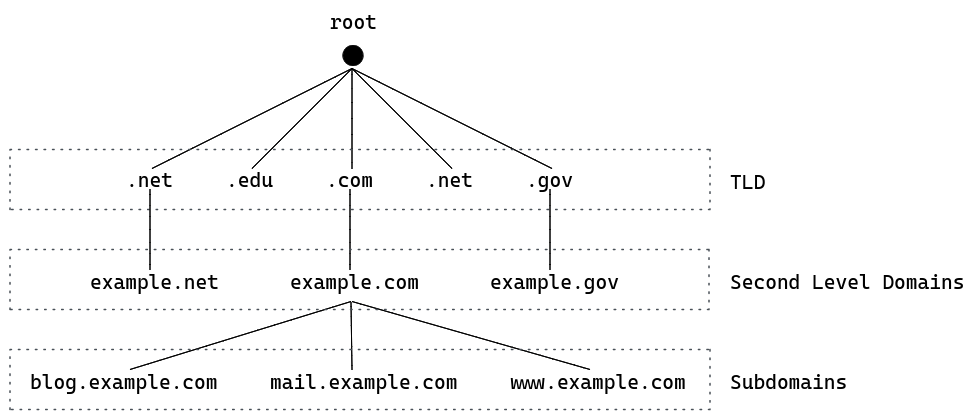
\includegraphics[width=\linewidth]{draws/dns-arch.png}
    \caption{Arquitectura de DNS.}
\end{figure}

Los nodos (dominios) son agrupados en zonas, las cuales pueden considerarse un área dentro del espacio de nombres. Siendo cada zona administrada por una organización o administrador determinado. La zonas son manejadas por servidores de autoridad, que pueden ser \textbf{primarios} (si la información de la zona tiene su origen fuera de DNS) o \textbf{secundarios} (la información tiene como origen un servidor primario, vía una transferencia de zona) [\cite{Vixie_2007}].

Cada nodo puede poseer registros (en inglés \textit{resource records} (RRs)). Estos son los que contienen toda la información DNS en dependencia de su nombre, tipo, clase o datos [\cite{rfc_1035}]. Cada RR tiene un TTL (\textit{time to live}), que indica que tiempo puede estar almacenada la información del registro en un servidor secundario, después de que este llegue a cero es necesario volver a obtener el registro del servidor autoritario primario.

\subsection{Tipos de Consultas DNS}

Como resultado de disponer de una base de datos distribuida, un servidor puede recibir una consulta que solo otro servidor puede responder. Así, una consulta DNS puede ser resuelta por los diferentes servidores que componen la jerarquía de nodos. Comenzando desde el nodo raíz hasta el servidor autoritario que debe contener la información requerida si esta existe.

\begin{figure}[!ht]
    \centering
    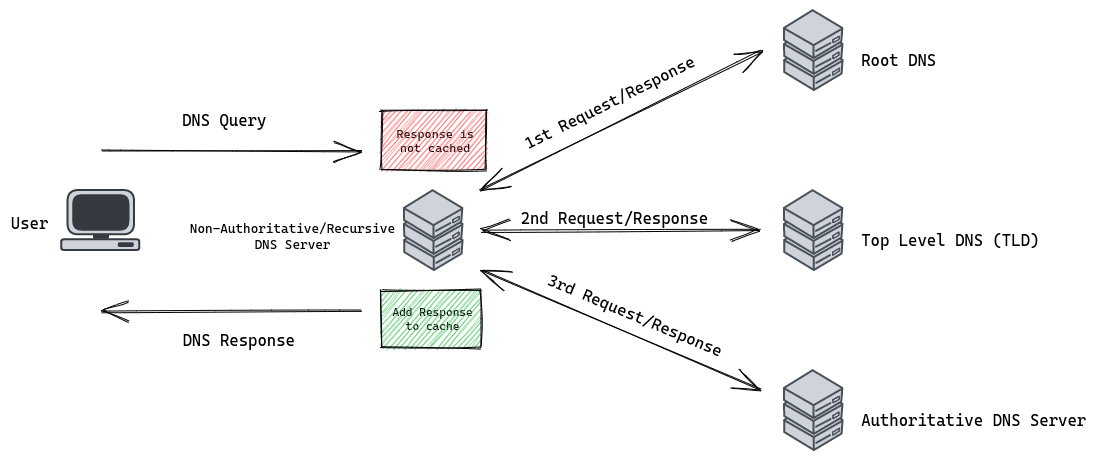
\includegraphics[width=\linewidth]{draws/dns-query.png}
    \caption{Resolución de una consulta DNS.}
\end{figure}

De forma estándar una consulta está compuestas por un dominio objetivo (\verb|QNAME|), un tipo (\verb|QTYPE|) y una clase (\verb|QCLASS|). El servidor DNS usa el \verb|QTYPE| y \verb|QCLASS| para dar respuesta a la consulta con el conjunto de RR relevantes. En adición a los registros retornados, el servidor puede apuntar a otro servidor de nombres que tiene información relevante para la consulta o útil para interpretar la información dada como respuesta.

Existen dos tipos de consultas (no confundir con \verb|QTYPE|), de acuerdo al proceso que realizan los servidores para dar la respuesta. Estas son recursivas e iterativas. Son dos aproximaciones distintas para resolver la obtención de información en una base de datos jerárquica y distribuida. DNS requiere la implementación de la solución iterativa y deja de manera opcional la recursiva [\cite{rfc_1034}].

En una consulta recursiva el cliente DNS provee el nombre de un host y el \textit{DNS Resolver} es el encargado de darle respuesta con un registro relevante o un mensaje de error en el caso que no fuera encontrado. El \textit{resolver} inicia esta consulta comenzando desde el servidor raíz, hasta que encuentre el servidor de nombres autoritario para la consulta, el cual contiene la dirección IP u otra información con la que dar respuesta.

Por otra parte, la consulta iterativa comienza cuando el cliente DNS provee el nombre de un host y el \textit{DNS Resolver} debe darle la mejor respuesta que tenga, dígase apuntarlo al servidor de nombres más probable de contener la respuesta a la consulta. Si el \textit{resolver} tiene el registro relevante para la consulta en su caché, este valor es dado como respuesta, sino el cliente es referido al servidor DNS raíz u otro servidor de nombres autoritario que sea más cercano a la zona deseada. Así, el cliente debe repetir la consulta al servidor al que fue referido.

\subsection{Registros y Extensibilidad}

Los registros DNS han ido evolucionando a lo largo de los años desde el diseño inicial del sistema. Diferentes RFCs (\textit{Request for Comments}) han ido añadiendo nuevos registros y dejando obsoletos otros. Los principales motivos para estos cambios es añadir nuevas funciones a DNS y mejorar la seguridad del sistema. Otro caso son tipos de registros que aún no son obsoletos pero están en desuso o no son usados por ninguna aplicación notable.

Los registros son el punto final de la jerarquía DNS, donde un nodo puede contener un conjunto de estos, que puede ser vacío. Ante una consulta resuelta por el nodo da como respuesta con un subconjunto de los RR que él mantiene.

Un RR esta conformado por diferentes campos. De forma general, tiene un propietario, que es el nombre de dominio dónde es encontrado, un tipo, algunos de los más comunes son \verb|SOA|, \verb|A|, \verb|NS|, \verb|MX|, \verb|CNAME|, y una clase que indica el protocolo al que pertenece y un TTL. Cada registro tiene finalmente un \verb|RDATA| dependiente de la clase y en ocasiones del tipo, por lo que puede contener información variada. Este puede ser un nombre de dominio, una dirección IP o incluso texto de propósito general, como es el caso del tipo \verb|TXT| [\cite{rfc_1464}].

\subsection{Seguridad}

Una vulnerabilidad de un sistema o una red es cualquier debilidad mediante la cual pueda comprometerse la información o el comportamiento del mismo. Múltiples amenazas pueden hacer uso de debilidades en un servidor DNS que no este configurado apropiadamente y realizar acciones malintencionadas.

DNS en su diseño inicial no esta orientado a la seguridad. Fue creado cuando el tráfico en internet era mucho menor a lo que es ahora y la seguridad no era una de las consideraciones principales. Consecuencia de ello, cuando un \textit{resolver} le envía una petición a un servidor autoritario de zona, no tiene como verificar la autenticidad de la respuesta que recibe. Solo es posible verificar que la dirección IP coincida, pero este no es un mecanismo lo suficientemente fuerte para garantizar la autenticidad, pues la dirección IP puede ser falsificada.

Como resultado de este diseño DNS, es vulnerable a muchos ataques. \textit{Cache poisoning} es una consecuencia directa de la ausencia de un mecanismo para verificar la autenticidad de una respuesta. Un \textit{resolver} puede almacenar en caché una respuesta que fue vulnerada, a partir de este punto responderá a la consulta posteriores con información comprometida, poniendo en peligro a los clientes. Otro riesgo es \textit{DNS Tunneling}, este se desarrolla cuando un atacante es capaz de ejecutar un malware que intercepte la comunicación entre el cliente y el \textit{resolver}. Dado que estas peticiones están autorizadas a pasar el cortafuegos, el atacante también puede pasar por este sin ser bloqueado [\cite{dns-tunneling}]. A la par existen amenazas que afectan este tipo de sistemas de forma general, principalmente ataques de denegación de servicios, ya sean DoS, DDoS (distribuidos) o DRDoS (reflexión distribuida) [\cite{dns-attacks}]. Un ataque de subdominios aleatorios también es un riesgo, consiste en realizar peticiones al servidor de dominios que no existen pero que pertenecen a la zona, gastando así el ancho de banda y los recursos de cómputo del servidor. Similar a este un ataque de NXDOMAIN tiene como objetivo vulnerar la caché de un \textit{resolver} o servidor autoritario, realizando muchas consultas de dominios que no existen, la respuesta a estas es un registro NXDOMAIN que queda almacenado en caché, así puede llenarse la caché, eliminando información relevante, lo cual causa una demora para resolver las consultas de los clientes reales [\cite{dns-attacks-ident-prot}].

Lógicamente, motivo de la importancia de DNS para las empresas y organizaciones con el auge del internet, fue necesario implementar mecanismos de seguridad que hicieran de DNS un sistema más seguro. En marzo de 2005 es publicado el RFC 4033 que propone un mecanismo, DNSSEC (\textit{Domain Name System Security Extensions}), para autenticar el origen de los datos y la integridad de estos ante una consulta. DNSSEC mejora la autenticación en DNS haciendo uso de firmas digitales basadas en criptografía de llave pública. Cada zona tiene un par de llaves pública y privada. El propietario de la zona hace uso de la llave privada para firmar la información DNS que envía. Mientras que la llave pública es usada por el \textit{resolver} para validar la información recibida [\cite{new-approach-dnssec}].

Aún existe un punto débil, y es como un \textit{resolver} puede verificar que la llave pública que esta recibiendo desde un servidor autoritario es auténtica. Para garantizar su autenticidad es usado el par de llaves del servidor padre, así se hace necesario que el padre y cada uno de los ancestros, hasta la raíz, tengan implementado DNSSEC. Afortunadamente desde el año 2010 el servidor raíz hace uso de DNSSEC, pero no todas las zonas en internet lo han adoptado aún [\cite{dnssec-icann}].

Otras vulnerabilidades de DNS son mostradas en la sección siguiente y específicamente como BIND las mitiga.  

\section{BIND 9}

BIND 9 (Berkeley Internet Name Domain versión 9) en un software de código abierto, mantenido oficialmente por el Internet Systems Consortium (ISC). Actualmente cuenta con tres ramas principales: Estable, Soporte-Extendido y Desarrollo. Esta implementado en C y su código disponible en GitLab\footnote{https://gitlab.isc.org/isc-projects/bind9}. Este es de los más consolidados en el mercado actual de soluciones DNS [\cite{dns-survey}; \cite{bind-usage}], con su surgimiento a inicios de la década de 1980 en la Universidad de California en Berkeley.

Posee un amplio abanico de características empleadas en el sistema DNS actual y es muy utilizado al ser primero en su tipo. Este ofrece tanto un servidor DNS autoritario como un DNS \textit{resolver}, así como un grupo de herramientas adicionales para la gestión del servicio DNS. Ambos servidores siguen prácticas de seguridad y ofrecen funcionalidades que garantizan su correcto funcionamiento al realizar el despliegue en cualquier red.

\subsection{DNS Autoritario}

El DNS autoritario tiene soporte para DNSSEC, lo cual permite ponerlo en producción con un alto esquema de seguridad y que nodos hijos puedan implementar DNSSEC por igual. Este servidor puede tener diferentes roles de acuerdo a la arquitectura usada en el despliegue. Estos roles son Primario, Secundario y Secundario Stealth. Esta arquitectura es escalable, es posible tener un servidor primario (maestro), como fuente de información para la zona, y uno o más servidores secundarios (esclavos). De esta forma los archivos de zona son actualizados en el servidor primario, mientras que los secundarios mantienen copias para responder a consultas.

La transferencia de información entre los servidores de la zona puede ser originada por el servidor primario ante un cambio. Dicho servidor envía un mensaje de tipo \verb+NOTIFY+ a los servidores secundarios, así estos son enterados de que deben realizar una transferencia de zona. Esta transferencia es configurable y puede ser realizada tanto de forma parcial (AXFR), como incremental (IXFR), haciendo uso de TSIG estándar como mecanismo de seguridad.

Las consultas de tipo \verb+ANY+ pueden obtener más información de la que envían, lo que las hace eficaces para efectuar DDoS. El servidor autoritario tiene un mecanismo para protegerse ante esta amenaza, retornando un conjunto predefinido de registros y no todos. BIND 9 usa \textit{rate-limiting} como mecanismo para prevenir ataques de amplificación (un tipo de RDDoS), este puede ser configurado en las opciones o en el ámbito de una vista. Los ataques de amplificación pueden ser evitados con las DNS \textit{Cookies} [\cite{rfc_7873}], estas permiten evitar IPs falsificadas en las consultas y como consecuencia que el servidor no sea involucrado en un ataque de reflexión.

Ante cambios en la configuración de las zonas es posible reiniciar el servidor usando la herramienta de línea de comandos \verb+rndc+ (\textit{remote name daemon control}). \verb+rndc+ permite cargar todas las zonas o especificar cuál, lo cual puede mejorar el tiempo de recarga de la configuración. Además se encarga de remover las zonas eliminadas al recargar la configuración. Esto es la forma más segura de efectuar el proceso, no es necesario reiniciar el servicio y la nueva información de las zonas es enviada a los servidores secundarios si existen.

\verb+dnstap+\footnote{\url{https://github.com/dnstap}} es una solución de código abierto para capturar y \textit{loguear} tráfico DNS. Es soportado por varios servidores DNS de código abierto, entre ellos BIND. Permite capturar el tráfico tanto de consultas como de respuestas del servidor con un impacto menor al \textit{logging} nativo de BIND. La información capturada es almacenada en formato binario, por lo que se ofrece para presentarla de forma legible la herramienta \verb+dnstap-read+. 

\subsection{DNS Resolver}

El DNS \textit{resolver} en BIND también posee funcionalidades que lo hacen muy potente y seguro. DNSSEC viene incorporado y se puede activar de manera sencilla. En caso que exista un problema con el DNSSEC del servidor autoritario puede ser ejecutado el \textit{resolver} con este deshabilitado, haciendo uso de \textit{Negative Trust Anchors} [\cite{rfc_7646}].

Uno de los aspectos más vulnerables y eficaces de los resolvers es la caché. El \textit{resolver} the BIND permite de forma flexible modificar los registros almacenados en caché. Esto puede resultar útil si los datos en caché son incorrectos o están desactualizados. Además, dispone de \textit{cache prefetch}, este mecanismo obtiene desde el servidor autoritario registros que son de frecuente acceso pero que tienen un TTL bajo, mejorando def forma efectiva los \textit{hits} en caché.

Para prevenir ataques DDoS el \textit{resolver} presenta dos opciones de configuración: \verb+fetches-per-zone+ y \verb+fetches-per-server+. Ambas limitan la cantidad de consultas a los servidores autoritarios que puedan estar bajo ataque y de esta forma mitigar la amenaza por la ruta del \textit{resolver}.

Una característica única en BIND es la posibilidad de configurar diferentes vistas en un mismo servidor. Esto permite mostrar a lo usuarios de una red interna y externa (como internet) diferente información DNS, manteniendo cierta información privada. También BIND, de forma particular, ofrece RPZ [\cite{rpz}] (\textit{Response Policy Zone}), estas son zonas diseñadas con un grupo especifico de reglas. Son especialmente usadas para bloquear el acceso a dominios que son conocidos por abuso o actividades ilegales.

\subsection{Alternativas}

Como fue mencionado en la Motivación, existen alternativas a BIND 9. En la tabla a continuación se muestra alguna de ellas.

\begin{table}[!ht]
    \centering
    \begin{tabular}{|l|c|c|c|c|c|}
    \hline
        Software & Pago & API HTTP & Web UI & Nube & Código Abierto \\ \hline
        BIND 9 & $\times$ & $\times$ & $\times$ & $\times$ & \checkmark \\ \hline
        PowerDNS & $\times$ & \checkmark & $\times$ & $\times$ & \checkmark \\ \hline
        CoreDNS & $\times$ & $\times$ & $\times$ & $\times$ & \checkmark \\ \hline
        Knot & $\times$ & $\times$ & $\times$ & $\times$ & \checkmark \\ \hline
        Amazon Route 53 & \checkmark & \checkmark & \checkmark & \checkmark & $\times$ \\ \hline
        DNS Made Easy & \checkmark & \checkmark & \checkmark & \checkmark & $\times$ \\ \hline
        Google Cloud DNS & \checkmark & \checkmark & \checkmark & \checkmark & $\times$ \\ \hline
        DNSimple & \checkmark & \checkmark & \checkmark & \checkmark & $\times$ \\ \hline
        NS1 & \checkmark & \checkmark & \checkmark & \checkmark & $\times$ \\ \hline
    \end{tabular}
    \caption{Comparativa de soluciones DNS.}
    \label{dns-comparative}
\end{table}

Tanto los servidores de código cerrado, como los de código abierto son mantenidos por instituciones. Los primeros poseen por lo general interfaces de usuario y son gestionados como SaaS (\textit{Software as a Service}). Permiten escalabilidad y acceso a personas sin conocimientos de administración de sistemas a la configuración del servidor DNS. Los proyectos abiertos son más orientados al perfil de administrador de sistemas, donde un conocimiento detallado de la tecnología es necesario.

En este escenario puede hacerse complejo para las organizaciones mantener una arquitectura DNS sin incurrir en gastos de licencia o de personal calificado. Se hace necesario constantemente la intervención de profesionales para modificar la configuración. Una ventaja de poseer el servidor en infraestructura propia y privada es que es más seguro que tenerlo expuesto a internet.

% https://doc.powerdns.com/authoritative/http-api/index.html
En el caso de PowerDNS\footnote{\url{https://github.com/PowerDNS/pdns}}, existe una API HTTP para manejar las zonas del DNS autoritario. Además acepta diferentes tipos de backends, incluyendo los archivos de configuración de BIND para las zonas. Por tanto una implementación para BIND, tentativamente sería aplicable a PowerDNS y otros productos de código abierto.

CoreDNS\footnote{\url{https://github.com/coredns/coredns}}, en su lugar, es muy flexible y la mayor parte de su funcionalidad es derivada de plugins. Actualmente, las instalación por defecto cuenta con más de 30 plugins, pero existen muchos externos y la posibilidad de escribir nuevos para funcionalidades concretas.

Knot\footnote{\url{https://gitlab.nic.cz/knot/knot-dns}} es un servidor DNS solo autoritario con un alto rendimiento, escrito en C. Soporta las características fundamentales del DNS actual, así como reconfiguración en tiempo de ejecución. El software esta orientado a sistemas operativos de tipo POSIX y su desarrollo va enfocado a las necesidades de la comunidad y usuarios donantes al proyecto.

En el grupo de SaaS se encuentra Amazon Route 53\footnote{\url{https://aws.amazon.com/route53/}} con características esenciales para el internet actual. Dispone de cortafuegos para el \textit{resolver}, control de recuperación ante fallos, flujo de tráfico basado en geoproximidad, latencia, salud y otras consideraciones. Como es de esperar, soporta DNSSEC y hace uso de una interfaz gráfica en la web que permite realizar la gestión DNS sin manejar código o archivos de configuración. También ubicado en su propio ecosistema, muy rico en soluciones, está Google Cloud DNS, con características semejantes a las ofrecidas por el producto de Amazon: IAM (\textit{Identity Access Management}), \textit{logging}, DNSSEC, zonas privadas, integración nativa con Kubernetes, y muchas otras.

Los demás servicios de pago como DNS Made Easy\footnote{\url{https://dnsmadeeasy.com/}}, DNSimple\footnote{\url{https://dnsimple.com/}} y NS1\footnote{\url{https://ns1.com}}, también ofrecen registro de nombres de dominio, API HTTP e interfaz web para su gestión. Los SaaS son especialmente útiles para empresas que posean un mercado estable y quieran dedicar menos tiempo a la gestión DNS. Además de mayor seguridad y margen de expansión haciendo uso de sistemas altamente escalables.

\section{Desarrollo Web}

Las opciones de tecnologías para el desarrollo web actual son bastante amplias. La mayoría de los lenguajes de alto nivel tienen \textit{frameworks} o bibliotecas que facilitan el desarrollo. En desarrollo \textit{front-end} JS/TS\footnote{\url{https://www.typescriptlang.org/}} es el estándar, para \textit{back-end}, las principales diferencias en desarrollo y producción son introducidas por el lenguaje usado. La mayoría de las soluciones existentes en Python, C\#, Java, JS/TS, Go son de código abierto y vienen cargadas de características para disímiles escenarios de implementación.

\subsection{Golang}

Go es un lenguaje compilado con tipado estático diseñado en Google, para el año 2007, por Robert Griesmen, Rob Pike y Ken Thompson. Fue desarrollado para afrontar los retos ingenieriles a los que se enfrentaban los ingenieros en Google. A día de hoy, desde su publicación en 2009, ha alcanzado una adopción masiva y empresas como Cloudflare, Dropbox, Meta, Microsoft, Netflix, PayPal, Twitter, Salesforce, Uber, entre otras, hacen uso de este lenguaje para servir millones de pedidos en escenarios de alta concurrencia con alta disponibilidad. [\cite{go-docs}]

La biblioteca estándar por si sola ofrece las herramientas necesarias para desarrollar una aplicación web. \textit{Encoding} y \textit{decoding} de JSON, validación de datos, implementación de cliente y servidor HTTP, sistema de plantillas HTML seguro contra inyecciones de código, \textit{drivers} para las bases de datos mas usadas, son algunas de las funcionalidades que vienen con el lenguaje.

Existen web frameworks de código abierto, enfocados en el rendimiento y el rápido prototipado, para ayudar en el desarrollo web. Gin\footnote{\url{https://github.com/gin-gonic/gin}}, Buffalo\footnote{\url{https://github.com/gobuffalo/buffalo}}, Echo\footnote{\url{https://github.com/labstack/echo}}, Flamingo\footnote{\url{https://github.com/i-love-flamingo/flamingo}} son algunos de ellos. También de parte de la comunidad podemos encontrar ORMs (\textit{Object Relational Mapper}) como GORM\footnote{\url{https://github.com/go-gorm/gorm}}, para la autenticación web Goth\footnote{\url{https://github.com/markbates/goth}}, con un número amplio de métodos [\cite{goth}], así como implementaciones de JWT (\textit{JSON Web Token}) en el lenguaje.

El método de concurrencia que usa Go es uno de los aspectos fundamentales al considerar el lenguaje. Las llamadas gorutinas (\textit{goroutines} en inglés) son un mecanismo poderoso de concurrencia, más ligeras que los hilos, con solo 2KB en tamaño. Un hilo puede tener cientos de gorutinas ejecutándose. La comunicación entre estas es a través de canales (\verb+chan+), vía de Go para recibir y enviar información entre las gorutinas.

Con la versión 1.18 de Go se añadió genericidad [\cite{go-generics}] al lenguaje, poderosa característica que permite ampliar la reusabilidad del código y la eficiencia durante el desarrollo. El manejo de memoria en Go, es realizado de forma automática por el recolector de basura. El impacto de este sobre el rendimiento es menor y añade más seguridad y portabilidad al software que el manejo manual de la memoria.

El lenguaje hace uso de paquetes para separar el código lo que ayuda a la separación de conceptos y hace uso de un desarrollo enfocado a bibliotecas. De esta forma diferentes proyectos pueden ser desarrollados sobre otros. La compilación en Go se realiza a un solo binario y es más rápida que en otros lenguajes compilados. Las dependencias se encuentran de forma explícita en el código lo que permite realizar la compilación y unión de estas de forma más rápida. En un escenario donde \verb+A.go+ depende de \verb+B.go+ y este de \verb+C.go+, pero \verb+A.go+ no de \verb+C.go+, el compilador primero compila \verb+C.go+, luego \verb+B.go+, y finalmente \verb+A.go+, adicionalmente para compilar \verb+A.go+ se usa \verb+B.go+, no \verb+C.go+ [\cite{go-deps}]. Esta aproximación disminuye considerablemente el tiempo de compilación en proyectos con muchas dependencias.

Para facilitar el desarrollo podemos encontrar de forma predeterminada en el lenguaje varias utilidades: manejo de dependencias, generación de documentación con ejemplos, formateo del código, automatización de tests y \textit{profiling}, son las principales. También es posible analizar los binarios puestos en producción a través de un servidor HTTP [\cite{go-pros-cons}].

\subsubsection{APIs con Go}

Como fue mencionado, existen diferente bibliotecas y frameworks para el desarrollo de servicios HTTP. Este entorno es bastante maduro pues el principal uso del lenguaje es escribir aplicaciones de \textit{back-end}.

Buffalo es un ecosistema para el desarrollo web, actualmente en su version 1.0.1 cuenta con herramientas para generar el la estructura inicial de un proyecto, un ORM con generación automática de modelos, migraciones y configuración para la base de datos. Viene listo para trabajar con tecnología front-end pero también tiene como opción generar un proyecto con el objetivo de servir una API REST HTTP. Podemos encontrar por defecto \textit{hot code reloading} y soporte para realizar \textit{testing}.
              
Echo se autoproclama de alto rendimiento, extensible y minimalista. Este framework dispone de forma predeterminada de un amplio número de \textit{middlewares} que cubren muchos escenarios comunes en el desarrolla de una API o servidor HTML, además de, TLS (\textit{Transport Layer Security}) de forma automática, control de direcciones IP de clientes e integración con cualquier sistema de plantillas. La documentación contiene un índice de referencias con guías paso a paso para diferentes soluciones que se pueden implementar sobre framework, siendo así un buen punto de consulta.

Flamingo es un framework bastante joven, cuenta con poco más de 300 estrellas en GitHub. Está más bien enfocado al desarrollo de aplicaciones \textit{full-stack} que a la implementacion de APIs. Dispone de un poderoso motor de plantillas, diseño orientado a microservicios y escalabilidad en el rendimiento. Además, posee un arsenal de características para la implementación de plataformas de comercio en línea, adaptables a las necesidades de negocio.

Finalmente Gin, con más de 63800 estrellas en GitHub es uno de los frameworks más usados. Semejante a los anteriores, ofrece alto rendimiento, soporte para \textit{middlewares} y extensión de estas, y manejo de errores. Gin captura errores  de pánico y se recupera de estos, de esta forma el servidor siempre esta disponible. El soporte para validación de JSON viene integrado, así como la renderización de plantillas.

Puede concluirse que Go tiene un ambiente con bastas opciones para el desarrollo web. Los frameworks, aunque algunos más consolidados que otros, comparten varias características comunes: extensibilidad, validación de datos, \textit{middlewares} y el alto rendimiento típico del lenguaje. Estas cualidades junto con las herramientas estándar que ofrece el lenguaje hace del desarrollo un proceso bien definido a la hora de afrontar un nuevo proyecto.

\subsection{Vue.js}

Vue.js\footnote{\url{https://github.com/vuejs/core}} es un framework progresivo de código abierto para crear interfaces de usuario en la web con Javascript. Es creado por Evan You después de trabajar para Google en varios proyectos con AngularJS. Vue tiene características similares a Angular, pero con una sintaxis más concisa y sencilla de usar. De igual forma ha adoptado ideas de otros frameworks y bibliotecas como React. [\cite{vue-docs}]

Ofrece un modelo de programación declarativo y basado en componentes que ayuda a desarrollar interfaces de usuario, tanto simples como complejas, de manera flexible. La comunidad ha desarrollado muchas bibliotecas opcionales que son activamente mantenidas, como son: Vue Router (enrutador para crear aplicaciones \textit{single-page}, SPA, por sus siglas en inglés), Pinia (biblioteca para manejo de estado), Vue Server Renderer (biblioteca para renderizado del lado del servidor), entre otras.

El framework ha ido cambiando de manera progresiva (como proclama su eslogan) y adoptando nuevas características. Con Vue 3 se introduce Compostion API como alternativa al estilo establecido por Options API. Ambos estilos son capaces de cubrir los casos de uso, sin embargo Option API esta desarrollada sobre Composition API. Por tal motivo, esta última ofrece más flexibilidad para crear patrones más específicos a la hora de organizar el código y reusar la lógica.

\hspace{-0.65cm}\begin{minipage}{0.5\textwidth}
    \begin{lstlisting}[basicstyle=\ttfamily\tiny, numbers=none, caption=Options API.]
<script>
export default {
// Properties returned from data() become reactive state
// and will be exposed on `this`.
data() {
    return {
    count: 0
    }
},

// Methods are functions that mutate state and trigger updates.
// They can be bound as event listeners in templates.
methods: {
    increment() {
    this.count++
    }
},

// Lifecycle hooks are called at different stages
// of a component's lifecycle.
// This function will be called when the component is mounted.
mounted() {
    console.log(`The initial count is ${this.count}.`)
}
}
</script>

<template>
<button @click="increment">Count is: {{ count }}</button>
</template>
    \end{lstlisting}
\end{minipage}
\begin{minipage}{0.5\textwidth}
    \begin{lstlisting}[basicstyle=\ttfamily\tiny, numbers=none, caption=Composition API.]
<script setup>
import { ref, onMounted } from 'vue'

// reactive state
const count = ref(0)

// functions that mutate state and trigger updates
function increment() {
    count.value++
}

// lifecycle hooks
onMounted(() => {
    console.log(`The initial count is ${count.value}.`)
})
</script>

<template>
    <button @click="increment">Count is: {{ count }}</button>
</template>
    \end{lstlisting}
\end{minipage}

\subsubsection{Reactividad}

La reactividad es una de las principales características de Vue. Con esta cada componente mantiene una referencia a sus dependencias reactivas. De esta forma es posible para el sistema saber cuando renderizar o cual componente renderizar.

En vainilla Javascript no es posible detectar cuando una variable local es leída o modifica. Vue hace uso de proxies (con objetos reactivos) o \textit{getters} y \textit{setters} (con \textit{refs}) para detectar dichos eventos y realizar el renderizado de la parte de la componente afectada.

\subsubsection{Enrutamiento} 

El enrutamiento en el lado del cliente es uno de los puntos fuertes de Vue. Permite crear SPAs que ofrecen una navegación más fluida al no cargar el HTML completo de la página para cada vista. La biblioteca Vue Router es oficialmente soportada por Vue y ofrece completa funcionalidad para implementar la navegación en el lado del cliente.

Las peticiones al servidor son realizadas de acuerdo a la componente que es cargada, dejando libre a este de tener que generar HTML. Por lo general, el servidor solo debe disponer de una API REST o similar para servir la información a la página web.

\subsection{Docker}\label{sec:docker}

Docker brinda la capacidad de empaquetar y ejecutar una aplicación en un entorno aislado llamado contenedor. Los contenedores son livianos y contienen todo lo necesario para ejecutar la aplicación, por lo que no usan las dependencias instaladas en el \textit{host}. Un contenedor es creado a partir de una imagen, y estas se pueden compartir fácilmente asegurando que todas las personas que la reciben obtengan una versión que funciona de la misma manera. Adicionalmente permite manejar la infraestructura de la misma forma que se manejan las aplicaciones, lo que disminuye el tiempo entre escribir el código y llevarlo a producción. [\cite{docker-docs}]

Docker hace especial uso de las características de Linux para el aislamiento de los contenedores, específicamente \verb|namespaces| para el aislamiento de los recursos del host y \verb|cgroups| para el control y limitación de esos recursos. A diferencia de una máquina virtual (MV) que realiza la virtualización sobre el hardware, un contenedor es un proceso corriendo en el sistema operativo, y como resultado se realiza la virtualización sobre este.

\begin{figure}[!ht]
    \centering
    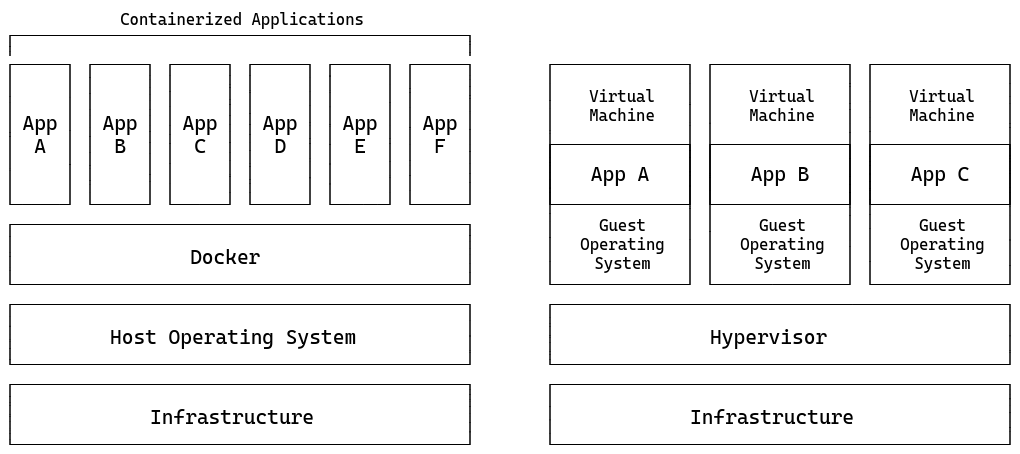
\includegraphics[width=\linewidth]{draws/cont-vs-vm.png}
    \caption{Comparación del funcionamiento de los contenedores y las MV. [\cite{docker-containers}]}
\end{figure}


La adopción de Docker es notable, existen alternativas como Podman, LXD, y Buildah, pero un número considerable de equipos y empresas escogen a Docker para la contenedorización de las aplicaciones [\cite{docker-usage}]. Este es de código abierto y gratis para proyectos de individuos, educación, pequeñas empresas y comunidades de código abierto.

El entorno en que se encuentra Docker es muy rico, dispone de DockerHub\footnote{\url{https://hub.docker.com}}, un sitio para almacenar imágenes, tanto públicas como privadas, lo que ofrece rápido acceso desde cualquier computadora a una imagen que haya sido subida. Estos repositorios son usados por las principales empresas distribuidoras de software, por lo que se pueden obtener productos de software con todas sus dependencias con solo una descarga. Válido mencionar que las principales tecnologías involucradas en este proyecto poseen imágenes en DockerHub: Golang, Node.js\footnote{\url{https://nodejs.org/en/}} para desplegar Vue.js, y los principales proveedores de DNS como BIND 9\footnote{\url{https://hub.docker.com/r/internetsystemsconsortium/bind9}}, PowerDNS\footnote{\url{https://hub.docker.com/u/powerdns}} y CoreDNS\footnote{\url{https://hub.docker.com/r/coredns/coredns/}}.

Las imágenes de Docker tienen una arquitectura por capas, una se construye sobre las otra. Así, si dos imágenes tienen una capa en común, dicha capa no se almacena de forma duplicada en disco y comparten ambas la misma. Los contenedores pueden persistir información en volúmenes, los cuales son sumamente portables, incluso entre sistemas operativos. La comunicación entre los servicios (contenedores) de Docker esta aislada al sistema, y se debe especificar los puertos que se necesiten exponer para dar acceso al exterior. Estos también pueden ser orquestados con Docker Swarm\footnote{\url{https://docs.docker.com/engine/swarm/}} o Kubernetes\footnote{\url{https://kubernetes.io/es/}}, lo que permite escalabilidad en producción acorde a las necesidades de cada servicio.

\subsubsection{Compose}

Compose es una herramienta para la definición y ejecución de aplicaciones con múltiples contenedores [\cite{docker-compose}]. Usa un archivo YAML como configuración, en el que se declaran los servicios, redes, volúmenes y otros objetos de Docker de los que va a hacer uso la aplicación. Es capaz de iniciar, detener y reiniciar contenedores, consultar el estado y los \textit{logs} de los servicios en ejecución, así como ejecutar comandos directamente sobre los servicios.      

Resulta de suma utilidad a la hora de desplegar múltiples servicios que estén relacionados en un proyecto, pues estos se alojan en una misma red privada, aislados de otros contenedores y el \textit{host}. Además, en esta red los servicios son localizables por su \textit{hostname} sin necesidad de conocer sus direcciones IP con anterioridad.


\chapter{Propuesta}\label{chapter:proposal}

A partir del estudio hecho en el capítulo anterior podemos asumir que sería beneficioso para las soluciones actuales de código abierto disponer de una API HTTP que permita la configuración de estos de forma programática. Facilitaría la integración con diferentes tipos de interfaces de usuario, ya sea web, de escritorio o una plataforma de terceros. Esta es una característica decisiva para la adopción de más usuarios, por ello los diferentes SaaS apuestan por ella y la ofrecen dentro de sus planes de pago.

De forma subyacente los diferentes servidores DNS están sujetos a la implementación de DNS propuesta en los RFC. Por tanto cada uno de los servidores de nombres debe tener el mismo punto de vista respecto al sistema. Poseer de un sistema de almacenamiento para persistir los diferentes conjuntos de RR en cada zona e implementar las características de DNS actual, tanto las requeridas como las opcionales. Estos puntos en común que deben compartir las diferentes implementaciones de servidores DNS sientan las bases para asumir los aspectos en los que sustentar la propuesta teórica de una API HTTP sobre ellos.

Como propuesta de solución a la implementación de una API para los diferentes softwares de servidores DNS autoritarios de código abierto, se propone un arquitectura en la que API tiene acceso al sistema de almacenamiento de la configuración DNS para su manejo. Además existe un medio de comunicación entendible por la API y el servidor DNS para desarrollar cualquier intercambio de información necesario.

\begin{figure}[!ht]
    \centering
    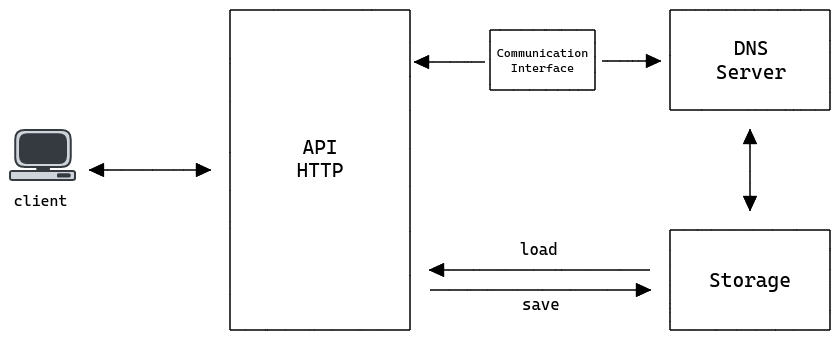
\includegraphics[width=\linewidth]{draws/proposal.png}
    \caption{Arquitectura de la propuesta.}
\end{figure}

La hipótesis teórica se basa en dos funciones: \verb+load+ para la lectura de los archivos de configuración desde un sistema de almacenamiento y \verb+save+ para la persistencia de los cambios realizados a dicho sistema. Estas funciones expuestas en una API HTTP, o similar, permiten realizar las funciones fundamentales de configuración sobre el servidor DNS.

En la sección 3.1 se describe el mecanismo carga de la configuración a través de la función \verb|load|. La sección 3.2 desarrolla el funcionamiento de \verb|save|, cómo esta asegura la correctitud de los cambios realizados en la configuración DNS y notifica al servidor DNS sobre estos.

\section{Lectura de la Configuración DNS}

Asumiendo que existe un servidor DNS autoritario $A$, con un sistema de persistencia en disco $S_A$. Sea $M_A$, la configuración del sistema DNS cargada por la API de $A$ y $r(S_A)$ una función capaz de leer y estructurar la información desde el sistema de almacenamiento $S_A$; se tiene la función \verb+load+ como se muestra a continuación.

\begin{algorithmic}
\Procedure{load}{$A$}
    \State $M_A \leftarrow r(S_A)$
\EndProcedure
\end{algorithmic}

\begin{figure}[!ht]
    \centering
    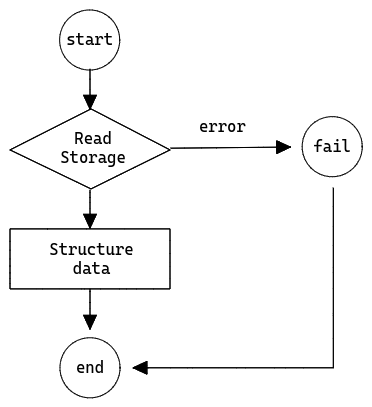
\includegraphics[width=0.5\linewidth]{draws/load.png}
    \caption{Diagrama de flujo para la función \textbf{load}.}
\end{figure}

Este procedimiento tiene como objetivo exponer cada una de las zonas con su conjunto de registros a la API. El mecanismo de lectura debe funcionar de acuerdo a como esta estructurada la información en el servidor DNS, archivos de texto plano, binarios o una base de datos externa. La estructura de datos resultante es manejada por la API y debe reflejar en todo momento el estado actual del servidor DNS.

\section{Escritura de la Configuración DNS}

Para definir \verb+save+, es necesario considerar que existe un mecanismo de comunicación $C_A$ entre el servicio de la API y $A$. Sean $h(C_A)$ una función que indica a $A$ que su configuración en $S_A$ ha sido modificada, $f(M_A, u)$ la función que almacena de forma estructurada en el almacenamiento de la API las modificaciones $u$ enviados a esta y $g(S_A, u)$ la función que persiste el conjunto de modificaciones $u$ de forma estructurada en el sistema de almacenamiento de $A$. Entonces, se define \verb+save+ de la siguiente manera.

\begin{algorithmic}\label{proc:save}
\Procedure{save}{$A$, $u$}
    \State $M_A' \leftarrow f(M_A, u)$
    \State $g(S_A, u)$
    \State $h(C_A)$
    \State $M_A \leftarrow M_A'$
\EndProcedure
\end{algorithmic}

\begin{figure}[!ht]
    \centering
    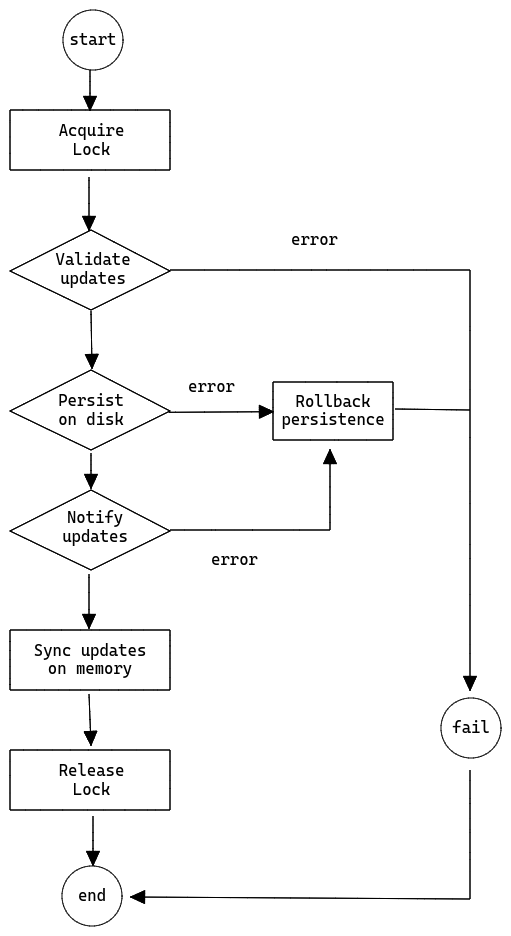
\includegraphics[width=0.6\linewidth]{draws/save.png}
    \caption{Diagrama de flujo para la función \textbf{save}.}
\end{figure}

Cuando se evalúa $f$ son realizadas las validaciones para garantizar que los cambios introducidos por $u$ son compatibles con el estado actual del servidor de nombres $A$. En caso positivo, la actualización introducida por $u$ es persistida. Posteriormente, se notifica al servidor DNS que puede recargar su configuración. Si los estados posteriores (invocación a $g$ y $h$) a la validación de $u$ ocurren sin errores, se actualiza la información en $M_A$ para sincronizarla con los cambios realizados al servidor autoritario $A$.

En caso de errores ambos sistemas deben quedar en el estado anterior a la ejecución de los cambios y la API debe retornar una respuesta indicando el error al completar el pedido. Para ello debe ser implementado un mecanismo que ejecute un \textit{rollback} de forma apropiada.

La interfaz de comunicación es explícitamente necesaria para notificar al servidor DNS de cambios. Por lo que cualquier tipo de protocolo factible para este fin es aceptable. En caso que el servidor de nombres sea capaz de detectar cambios en su configuración de forma autónoma en tiempo de ejecución, la invocación a $h$ puede ser omitida en la implementación.

\chapter{Detalles de Implementación y Experimentos}\label{chapter:implementation}

Con el objetivo de llevar a cabo la experimentación en la implementación de una API para los servidores DNS de código abierto, se tomó como software representativo BIND 9. En este capítulo se explican sus características principales que interactúan en la propuesta y la implementación de las funciones \verb|load| y \verb|save| sobre él.

En el presente capítulo se discutirán primeramente las características del sistema de almacenamiento que usa BIND para almacenar la configuración y las zonas del servidor DNS. Luego, en la sección 4.2, el mecanismo mediante el cual se notifica a BIND que ha sido modificado sus sistema de configuración, para que así pueda reflejar los cambios en tiempo de ejecución.

En las secciones posteriores, de la 4.3 a la 4.5, se describe como fueron desarrolladas la funciones de la propuesta y qué alternativas fue necesario tomar en su implementación. También se muestran las principales consideraciones para manejar errores ante los pedidos y cómo garantizar la sincronización entre los datos que maneja la API y el servidor de nombres.

En la sección 4.6, se discute el despliegue de los servicios con Docker y Compose. Finalmente, se plantean los experimentos realizados para verificar el correcto funcionamiento de la implementación y se discuten sus resultados.

\section{Sistema de Almacenamiento}\label{sec:bind-storage}
BIND usa como sistema de almacenamiento para el servidor DNS archivos de texto plano. En estos archivos se almacena tanto la configuración del servidor autoritario o secundario, como los archivos de zona con sus registros. En la imagen de Docker de BIND basada en Ubuntu\footnote{\url{https://hub.docker.com/r/ubuntu/bind9}} se pueden encontrar los archivos de configuración y de zona en los directorios \verb+/etc/bind+ y \verb+/var/lib/bind+ respectivamente.

\begin{lstlisting}[frame=single, numbers=none, caption=Contenido del directorio \textbf{/etc/bind}.]
$ ls /etc/bind
bind.keys  db.0  db.127  db.255  db.empty  db.local  named.conf
named.conf.default-zones  named.conf.local  named.conf.options
rndc.key  zones.rfc1918
\end{lstlisting}

El fichero principal de configuración para BIND es \verb+named.conf+, desde él se importan con la directiva \verb+include+ los demás ficheros de configuración (\verb|named.conf.options|, \verb|named.conf.local| y \verb|named.conf.default-zones|) que se encuentran en el directorio. Así, la configuración puede ser dividida en diferentes archivos, facilitando su mantenibilidad y legibilidad.

El archivo \verb+named.conf.options+ tiene las opciones globales que son usadas al iniciar el servicio. Estas son ubicadas entre llaves en el cuerpo de la declaración \verb+options+. La gramática está disponible online en el manual de administrador para BIND\footnote{\url{https://bind9.readthedocs.io/en/v9_18_8/reference.html\#namedconf-statement-options}}. En este se manejan los aspectos fundamentales de DNS, \textit{caching}, logging a través de \verb+dnstap+, así como la configuración relacionada a DNSSEC. En este espacio también son definidas las listas de control de acceso (ACL, por sus siglas en inglés), que permiten restringir el acceso al servidor basado en la dirección IP del host que hace la petición. BIND dispone de gran granularidad al poder definir un ACL para cada uno de diferentes tipos de consultas que acepta el servidor.

El fichero \verb+named.conf.local+ contiene la configuración local para el servidor DNS y es donde se declaran las zonas que este va a manejar. En este también se puede hacer uso de la directiva \verb+include+, para importar otros ficheros que declaran zonas usualmente, como es el caso de \verb+zones.rfc1918+.

Una zona es definida con un nombre, una clase (por defecto \verb+IN+, por \verb+Internet+) y un cuerpo que contiene un conjunto de opciones para la zona. Dentro de estas opciones es requerido definir su tipo con la palabra clave \verb+type+. Cada tipo tiene una gramática distinta de acuerdo a las opciones que admite.

La zona dentro de sus opciones permiten definir diferentes ACL, similar a las opciones globales. Cada zona puede tener su política para manejar actualizaciones en tiempo de ejecución. Específicamente, la opción \verb+allow-update+ maneja mediante una ACL quien pude actualizar registros en una zona. De igual forma, \verb+update-policy+ permite controlar quien modifica la zona basada en la identidad del solicitante, la identidad es determinada por la clave que firmó el pedido, usando TSIG o SIG(0). Estos dos mecanismos para controlar el acceso se definen de forma excluyente y el segundo solo puede ser usado en zonas de tipo primario (\verb+primary+ o \verb+master+).

Los otros ficheros ubicados en \verb+/etc/bind+, son \verb+bind.keys+ y el grupo de \verb+db.*+. El primero tiene como objetivo sobreescribir las claves públicas (\textit{trust anchors}) que usa BIND para DNSSEC. Los segundos son empleados para indicar la zona del \textit{host} y la interfaces de \textit{loopback} y \textit{broadcast}. Estos son cargados directamente por \verb+named.conf.default-zones+.

\begin{lstlisting}[frame=single, numbers=none, caption=Contenido del fichero \textbf{named.conf.default-zones}]
$ cat /etc/bind/named.conf.default-zones
// prime the server with knowledge of the root servers
zone "." {
    type hint;
    file "/usr/share/dns/root.hints";
};

// be authoritative for the localhost forward and reverse zones,
// and for broadcast zones as per RFC 1912

zone "localhost" {
    type master;
    file "/etc/bind/db.local";
};

zone "127.in-addr.arpa" {
    type master;
    file "/etc/bind/db.127";
};

zone "0.in-addr.arpa" {
    type master;
    file "/etc/bind/db.0";
};

zone "255.in-addr.arpa" {
    type master;
    file "/etc/bind/db.255";
};
\end{lstlisting}

\section{Comunicación con el servidor DNS}\label{section:comm-bind}

Cuando BIND sufre cambios en los ficheros de configuración estos no son detectados y reflejados en tiempo de ejecución. Debe reiniciarse el servicio o notificarlo de que ha ocurrido una actualización. La alternativa más eficiente es la segunda y \verb+rndc+ es la herramienta recomendada para este proceso.

\verb+rndc+ se comunica con el servidor de nombres a través de una conexión TCP, enviando comandos con una firma digital. La versión actual utiliza como algoritmos de autenticación HMAC-MD5 (por compatibilidad), HMAC-SHA1, HMAC-SHA224, HMAC-SHA256 (por defecto), HMAC-SHA384, y HMAC-SHA512. Estos utilizan una clave secreta compartida en cada lado de la conexión, lo cual provee de autenticación de tipo TSIG para la petición del comando y la respuesta del servidor. \verb+rndc+ utiliza una archivo de configuración para determinar cómo conectarse al servidor y el algoritmo y llave a emplear en la autenticación.

Para indicar cambios en los archivos de BIND con \verb|rndc| están disponibles los comandos \verb|reconfig| y \verb|reload|. El primero es empleado para notificar de una actualización en la configuración (\verb|named.conf| o sus dependencias) de BIND, por tanto, si una nueva zona es añadida BIND lo detectará. A pesar de cargar las nuevas zonas, \verb|reconfig| no percibirá cambios en las zonas. Para detectar cambios en la zona es necesario usar \verb|reload| o, de forma más específica, \verb|reload <zone-name>|. Especificando la zona se agiliza el proceso en servidores que tengan un alto volumen de zonas, evitando verificar zonas innecesariamente.

\begin{table}[!ht]
    \centering
    \begin{tabular}{|l|l|}
    \hline
        \textbf{Evento} & \textbf{Comando} \\ \hline
        Nueva zona & \verb|reconfig| \\ \hline
        Modificar zona & \verb|reload <zone-name>| \\ \hline
        Eliminar zona & \verb|reconfig| \\ \hline
    \end{tabular}
    \caption{Subcomando de \textbf{rdnc} apropiado para cada evento.}
    \label{table:rndc-event}
\end{table}

En las opciones de conexión de \verb|rndc| puede ser especificada la dirección IP del servidor de BIND al que conectarse. Siendo así, es posible instalar \verb|rdnc| en el ambiente de la API y especificar la dirección de BIND en el contenedor. Pero dado que la instalación de BIND viene con \verb|rndc| por defecto, es más factible invocar este de forma programática a través de Docker. Con este fin, se implementó un método que ejecutase un comando en el contenedor remoto, tomando como referencia la implementación del comando \verb|docker exec|\footnote{\url{https://github.com/docker/cli/blob/1163b4609978e0e6f2b2629b59c4a62d348e1466/cli/command/container/exec.go\#L99}} y en base a él los métodos \verb|Reconfig| y \verb|ReloadZone|.

\begin{lstlisting}[frame=single, language=Go, caption=Métodos para actualizar a BIND con los cambios en sus archivos.]
func (bs *BindService) exec(command ...string) error {
    if _, err := bs.DockerCli.ContainerInspect(bs.ctx, bs.ContainerId); err != nil {
        return err
    }

    execCreateConfig := &types.ExecConfig{
        User:         "bind",
        Privileged:   false,
        Tty:          false,
        AttachStdin:  false,
		AttachStderr: true,
        AttachStdout: false,
		Detach:       false,
        DetachKeys:   "",
        Env:          []string{},
        WorkingDir:   "/",
        Cmd:          command,
    }

    response, err := bs.DockerCli.ContainerExecCreate(bs.ctx, bs.ContainerId, *execCreateConfig)
    if err != nil {
        return err
    }
    if response.ID == "" {
        return errors.New("exec ID empty")
    }

    execStartConfig := &types.ExecStartCheck{
        Detach: execCreateConfig.Detach,
        Tty:    execCreateConfig.Tty,
    }

    if err := bs.DockerCli.ContainerExecStart(bs.ctx, response.ID, *execStartConfig); err != nil {
        return err
    }

    return nil
}

// Runs `rndc reconfig` in the BIND server.
// Reloads the configuration file and loads new zones, but does not reload existing zone files even if they have changed.
func (bs *BindService) Reconfig() error {
	return bs.exec("rndc", "reconfig")
}

// Runs `rndc reload {zone}` in the BIND server
func (bs *BindService) ReloadZone(zone string) error {
	return bs.exec("rndc", "reload", zone)
}
\end{lstlisting}

\section{Lectura de la Configuración DNS}

Con el fin de implementar la función \verb+load+ sobre el sistema de almacenamiento de BIND se hace necesario \textit{parsear} estos archivos de texto plano. Se requiere de un \textit{parser} para los archivos que contienen registros y otro para los archivos de configuración, específicamente \verb+named.conf.local+, que es el que usualmente contiene las zonas añadidas por los administradores del servidor.

El proceso de \textit{parsing} permite estructurar la información en texto plano tanto al leerla como al escribirla a disco. La gramática para los archivos de configuración está completamente definida en la documentación de BIND y está sujeta a los cambios que introduzca ISC en el software. En el caso de los archivos de registros no es tan sencillo, se rigen por DNS y este es un sistema en constante cambio, son añadidos nuevos tipos de registros o especificaciones, por lo que la gramática puede cambiar en un futuro. Definirla sobre los tipos más comunes y dejar como alternativa su extensibilidad es la opción más factible en este proyecto.

Para la implementación de los \textit{parsers} fue empleada la biblioteca de Go, Participle\footnote{\url{https://github.com/alecthomas/participle}}. Esta hace uso de la genericidad en el lenguaje para la definición de los \textit{parsers} y genera un \textit{parser} de descenso recursivo con \textit{backtracking} a partir de la gramática de entrada. La gramática es definida de forma declarativa en las etiquetas (\verb|parser|) de las estructuras que la conforman y lo tokens son almacenados en el campo al que referencian.

El \textit{parser} resultante para los archivos de zona, de forma simplificada, es el siguiente:

\begin{lstlisting}[frame=single, language=Go, escapechar=!, caption=Implementación en Go del \textit{parser} para los archivos de zona.]
import (
    "github.com/alecthomas/participle/v2"
	"github.com/alecthomas/participle/v2/lexer"
)

var (
    ZoneLexer = lexer.MustSimple([]lexer.SimpleRule{
        {Name: "Directive", Pattern: `\$(ORIGIN|TTL)`},
        {Name: "Keyword", Pattern: `@|IN`},
        {Name: "RType", Pattern: `SOA|NS|A|MX|TXT|CNAME`},
        {Name: "Origin", Pattern: `[a-zA-Z][\w\-]*\.[a-zA-Z]+`},
        {Name: "Name", Pattern: `[a-zA-Z][\w\-]*`},
        {Name: "Ttl", Pattern: `\d+[hdw]`},
        {Name: "Ipv4", Pattern: `\d{1,3}\.\d{1,3}\.\d{1,3}\.\d{1,3}`},
        {Name: "Uint", Pattern: `\d+`},
        {Name: "String", Pattern: `"[^"\n]*"`},
        {Name: "Punct", Pattern: `[\.\(\)]`},
        {Name: "Comment", Pattern: `;[^\n]*\n+`},
        {Name: "Whitespace", Pattern: `[ \t\r]+`},
        {Name: "NewLine", Pattern: `[\n]+`},
    })
    ZoneParser = participle.MustBuild[DomainConf](!\label{line:parser}!
        participle.Lexer(ZoneLexer),
        participle.Union[Record](NSRecord{}, ARecord{}, MXRecord{}, TXTRecord{}, CNAMERecord{}),!\label{line:union-gen}!
        participle.Elide("Whitespace", "Comment"),
        participle.Unquote("String"),
        participle.UseLookahead(2),
    )
)

type ZoneConf struct {
	Origin    string     `parser:"'$ORIGIN' @Origin '.' NewLine" json:"origin"`
	Ttl       string     `parser:"'$TTL' @Ttl NewLine" json:"ttl"`
	SOARecord *SOARecord `parser:"@@ NewLine" json:"soaRecord"`
	Records   []Record   `parser:"@@*" json:"records"`
}

type Record interface {
    // Omitted for brevity
}

type SOARecord struct {
	NameServer string `parser:"'@' 'IN' 'SOA' @Name" json:"nameServer"`
	Admin      string `parser:"@Name" json:"admin"`
	Serial     uint   `parser:"'(' @Uint" json:"serial"`
	Refresh    uint   `parser:"@Uint" json:"refresh"`
	Retry      uint   `parser:"@Uint" json:"retry"`
	Expire     uint   `parser:"@Uint" json:"expire"`
	Minimum    uint   `parser:"@Uint ')'" json:"minimum"`
}

type NSRecord struct {!\label{line:ns}!
	Type       string `parser:"'@' 'IN' @'NS'" json:"type"`
	NameServer string `parser:"@Name NewLine" json:"nameServer"`
}

type ARecord struct {
	Name string `parser:"@Name" json:"name"`
	Type string `parser:"'IN' @'A'" json:"type"`
	Ip   string `parser:"@Ipv4 NewLine" json:"ip"`
}

type MXRecord struct {
	Type        string `parser:"'@' 'IN' @'MX'" json:"type"`
	Priority    uint   `parser:"@Uint" json:"priority"`
	EmailServer string `parser:"@Name NewLine" json:"emailServer"`
}

type TXTRecord struct {
	Type  string `parser:"'@' 'IN' @'TXT'" json:"type"`
	Value string `parser:"@String NewLine" json:"value"`
}

type CNAMERecord struct {
	SrcName string `parser:"@Name 'IN'" json:"srcName"`
	Type    string `parser:"@'CNAME'" json:"type"`
	DstName string `parser:"@Name NewLine" json:"dstName"`
}
\end{lstlisting}

Como los diferentes tipos de registros (excluyendo a \verb|SOA|, por conveniencia siempre el primero) pueden encontrarse indistintamente en un archivo de zona, el orden de estos no es relevante, solo la información contenida acorde al tipo. En la línea~\ref{line:union-gen} se captura este comportamiento haciendo uso de la genericidad que ofrece el lenguaje. Por esta vía es posible declarar una producción en la gramática de la forma \verb+Record -> NSRecord | ARecord | MXRecord | TXTRecord | CNAMERecord+. El nodo raíz del AST (\textit{Abstract Syntax Tree}) es la estructura usada como tipo genérico en la construcción del \textit{parser} (línea~\ref{line:parser}), y en este caso particular, es la base para la información del archivo de zona. Aquí es declarado que todo archivos de zona contiene \verb+$TTL+, \verb|$ORIGIN|, \verb|SOA| y un \textit{slice} de \verb|Record|.

Tomando como ejemplo la estructura \verb+NSRecord+ (línea~\ref{line:ns}), esta va a consumir una cadena con una forma similar a \verb|@ IN NS <Name>|. Como resultado, va a almacenar en \verb|Type| el valor de tipo \verb|string| \verb|"NS"|. Luego declara que en el campo \verb+NameServer+ se va almacenar un token que coincida con el tipo \verb+Name+ del \textit{lexer} y consumir un salto de línea.

Una ventaja notable de poder representar la gramática en las etiquetas de las estructuras es que es consistente con la sintaxis usada para la serialización por defecto de estructuras en Go. Así se puede mantener en cada uno de los atributos el proceso de \textit{parsing} relacionado al \textit{token} que va almacenar, y junto ello, la etiquetas usadas para serializar y deserializar las estructuras al ser enviadas por la red.

% Así se puede mantener en la misma estructura que almacena los tokens resultado del proceso de \textit{parsing} la declaración de los campos correspondientes cuando se serialicen y deserialicen las estructuras al ser transmitidas por la red.

La implementación de la función \verb|load| se puede dividir en dos partes. La primera, \textit{parsear} la configuración (\verb|/etc/bind/named.conf.local|) de BIND para detectar todas las zonas disponibles y una segunda, en la que para cada zona encontrada se \textit{parsea} el archivo (campo \verb|file|) al que esta refiere.

\begin{lstlisting}[frame=single, language=Go, caption=Implementación de la función \textbf{load} para BIND.]
func (bs *BindService) Load() {
	var err error

	bs.BindConf, err = bs.parseBindConf(Service.ZonesFilePath)
	if err != nil {
		log.Fatal(err)
	}

	bs.Domains = make(map[string]*parser.DomainConf)

	for _, zone := range Service.BindConf.Zones {
		filename := zone.File[strings.LastIndex(zone.File, "/")+1:]

		zConf, err := Service.parseDomainConf(setting.Bind.LibPath + filename)
		if err != nil {
			log.Printf("Error loading %s: %s\n", filename, err)
			continue
		}

		Service.Domains[zConf.Origin] = zConf
	}
}
\end{lstlisting}

Este método es invocado al inicio del sistema y en caso de error al cargar la configuración de BIND se detiene la ejecución y se reporta. Si una zona contiene errores sintácticos es omitida a la hora de cargarla y el error es reportado. Solo son servidas zonas listadas en la configuración de BIND y que no contengan errores de sintaxis.

Las estructuras de datos resultantes almacenadas en \verb|BindService.BindConf| y \verb|BindService.Zones|, contienen la información que refleja el estado actual del servidor de nombres. El primero es el AST resultante de \textit{parsear} la configuración y el segundo, un mapa del nombre de cada zona al respectivo AST de su archivo que contiene el conjunto de RR.

\subsection{Almacenamiento en Memoria vs Disco}

Para la solución, inicialmente fue considerada cargar la configuración del servidor DNS a una base de datos. Dicha solución fue desechada en favor de almacenarla en memoria. La principal desventaja de esto es tener que implementar algunos mecanismos de validación que pueden ser declarados de forma relativamente sencilla con SQL. Pero trae varias ventajas consigo, la primera, y más importante, es no tener dos fuentes de verdad (base de datos de la API y base de datos del servidor DNS). De esta forma cada vez que se inicie la API se garantiza que la información que sirve está sincronizada con la configuración del servidor DNS. En última instancia el servidor de nombres es quien debe tener la información precisa pues es quien provee el servicio DNS. Además, se pude obtener menores valores de latencia, dado que el acceso a valores aleatorios en memoria es mucho más rápido que en disco (HDD o SSD)[\cite{jacobs2009pathologies}].

\section{Escritura de la Configuración DNS}

La información resultante del proceso de \textit{parsing} puede ser modificada y escrita a disco sin inconvenientes, permitiendo actualizar los archivos de configuración del servidor DNS de forma directa sin afectar su funcionamiento. Este proceso puede resumirse en tomar el AST resultante, llevarlo a una cadena de texto, similar a la que tuvo como origen, y escribir dicha cadena al fichero de configuración.

Como indica la función \verb+save+, es necesario mantener actualizada la copia de la configuración en memoria, esto evita tener que \textit{parsear} el archivo de configuración en modificaciones posteriores. Así se realiza el \textit{parsing} una sola vez al iniciar el sistema, posteriormente solo las escrituras del AST al archivo correspondiente.

En la propuesta, \verb|save| recibe como parámetros un servidor de nombres $A$ y una actualización a aplicar $u$. Dicha actualización puede ser uno de diferentes eventos, ya definidos en la Tabla \ref{table:rndc-event}, donde la modificación de una zona puede ser de forma específica añadir, modificar o eliminar uno de los registros de la zona.

Por tanto $u$, puede verse como un elemento de un conjunto de posibles eventos, y sería necesario verificar antes de procesar $u$ dentro de \verb|save| qué tipo de evento es el recibido. Una implementación que cubra esta lógica puede comprometer la legibilidad de \verb|save|, dado que genera código espagueti, además de resultar en una función más difícil de mantener y comprobar. Además, se debe tener en cuenta que no todas las modificaciones a la configuración requieren modificar la misma cantidad de archivos o invocar el mismo comando de \verb|rndc|. En el caso de añadir una nueva zona, es necesario modificar la configuración del servidor, así como el archivo de la nueva zona, mientras que al modificar la zona, solo se modifica el archivo de zona, y, como se analizó en \ref{section:comm-bind}, los comandos de \verb|rndc| a usar en cada caso son distintos.

Como consecuencia de esto, en la implementación se decide dividir \verb|save| en un conjunto de funciones (ver Figura \ref{fig:split-save}), que siguen cada uno de los estados que esta define, pero que manejan cada tipo de evento por separado. Adicionalmente, cada una de estas funciones está directamente relacionada con un punto final de la API.

\begin{figure}[!ht]
    \centering
    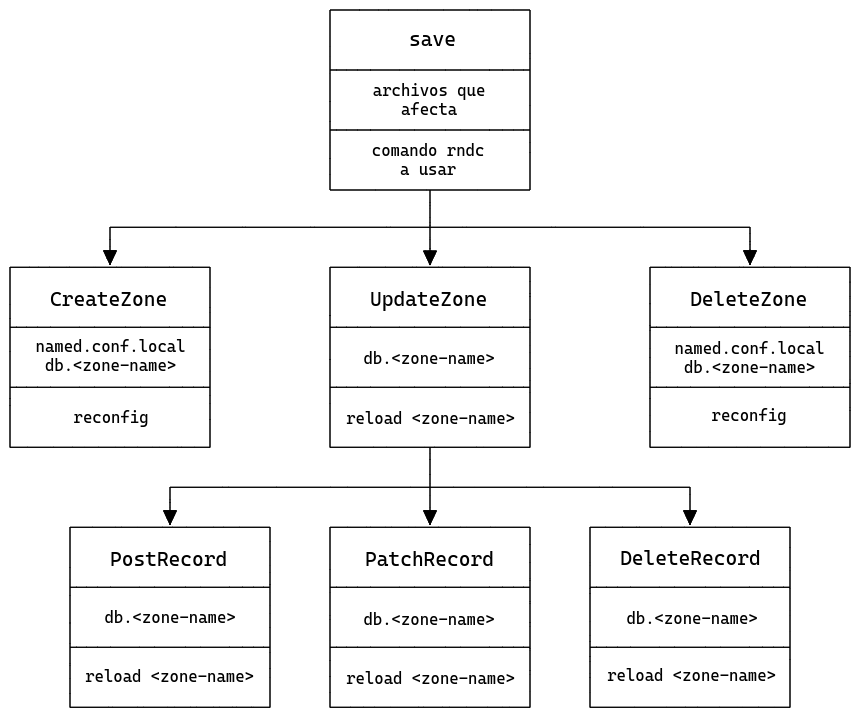
\includegraphics[width=\linewidth]{draws/split-save.png}
    \caption{Funciones que siguen el diseño de \textbf{save} para dividir la lógica. Cada una afecta diferentes archivos en la configuración de BIND 9 y usa un subcomando específico de \textbf{rndc} para actualizar en tiempo de ejecución el servidor de nombres.}
    \label{fig:split-save}
\end{figure}

Un cambio en la configuración por una función derivada de \verb|save| es originado por una invocación a los puntos finales de la API. Por tanto, cabe la posibilidad de que se traten de realizar de forma concurrente en memoria. Siendo así, se hace necesario limitar el acceso concurrente de escritura para evitar la corrupción de los datos haciendo uso de una instancia de \verb|sync.Mutex|. Cuando una modificación es recibida por la API, la función a ser invocada toma el control sobre este bloqueo, realiza la escritura en disco y memoria y luego lo libera.

La función principal del bloqueo es mantener la consistencia entre la información que se encuentra en memoria y en disco, asegurando que cada escritura en memoria tenga su sucesiva escritura en disco. El AST puede implementar su propio mecanismo para manejar el acceso concurrente en memoria, de igual forma se puede hacer a la hora de implementar la escritura en los archivos de configuración del disco. Sin embargo, estos dos por separado no garantizan la sincronización memoria-disco ante el acceso concurrente a la API. Además, es importante poder recuperarse de un error de escritura en disco, sin corromper la información en memoria.


Las zonas en los servidores DNS primarios son consideradas zonas de inicio de autoridad. Estas son la fuente de información para el servidor maestro y sus esclavos. Son representadas por un registro de tipo \verb|SOA| (\textit{Start Of Authority}) que contiene información administrativa y de importancia para los servidores secundarios. Los diferentes campos que contiene indican cada qué tiempo los servidores secundarios deben consultar al primario por actualizaciones, cada qué tiempo consultar por cambios en el número de serie y después de qué intervalo detenerse los esclavos en caso de fallo en el maestro. Un aumento en el número de serie indica a los servidores secundarios que ha ocurrido una actualización en la zona y por tanto se debe iniciar una transferencia.

\begin{lstlisting}[frame=single, numbers=none, caption=Ejemplo de zona con \textit{SOA}.]
$ORIGIN example.com.
$TTL 86400
@   IN  SOA     ns.example.com. admin@example.com (
        2022110300  ;Serial
        7200        ;Refresh
        3600        ;Retry
        1209600     ;Expire
        3600        ;Negative response caching TTL
)
\end{lstlisting}

Por tanto, es de vital importancia para el funcionamiento del servicio DNS que el número de serie sea incrementado en cada modificación a la zona, a pesar de que se pueda enviar una consulta de tipo \verb|NOTIFY| a los esclavos para alertar de una transferencia de zona. El número de serie es un entero positivo que indica la versión de la copia original de la zona, por lo general se puede usar como valor la fecha de cambio más dos dígitos para el caso en el que ocurran múltiples modificaciones el mismo día.

De esta forma, en la implementación es realizada la actualización de la versión de la zona cada vez que se persisten cambios en la configuración DNS.

\begin{lstlisting}[frame=single, language=Go]
// Generates a new serial for the SOA record.
// Generated serials follows the format YYYYMMDDNN where NN is a two digits identifier.
func (zc *ZoneConf) UpdateSerial() {
    now := time.Now().UTC()
    newSerial := uint(now.Year()*1_000_000 + int(now.Month())*10_000 + now.Day()*100)
    if zc.SOARecord.Serial >= newSerial {
        zc.SOARecord.Serial = zc.SOARecord.Serial + 1
    } else {
        zc.SOARecord.Serial = newSerial
    }
}
\end{lstlisting}

Según los aspectos definidos en esta sección, se muestra a continuación la función \verb|CreateZone|, una de las mencionadas en la Figura \ref{fig:split-save} y que refleja el comportamiento de \verb|save| y, de forma general, el conjunto de funciones en que está dividida.

\label{func:create-zone}
\begin{lstlisting}[frame=single, language=Go, escapechar=|, caption=Ejemplo de la función que añade una nueva zona al servidor DNS.]
func (bs *BindService) CreateZone(data *schemas.DomainData) (*parser.ZoneConf, error) {
    // Get write access to the filesystem and release it when done
    bs.Mutex.Lock()
    defer bs.Mutex.Unlock()

    // Validate that the new zone is not defined already 
    if _, ok := bs.Zones[data.Origin]; ok {
        return nil, fmt.Errorf("zone %s exists already", data.Origin)
    }

    // Create the new zone from received data
    zConf := &parser.ZoneConf{
        Origin: data.Origin,
        Ttl:    data.Ttl,
        SOARecord: &parser.SOARecord{
            NameServer: data.NameServer,
            Admin:      data.Admin,
            Refresh:    data.Refresh,
            Retry:      data.Retry,
            Expire:     data.Expire,
            Minimum:    data.Minimum,
        },
        Records: []parser.Record{},
    }

	bindConf := *bs.BindConf

	if err := bindConf.AddZone(zConf); err != nil {
		return nil, err
	}

    // Write new changes to BIND files and rollback on error
	rollbackZConf, err := zConf.WriteToDisk(zConf.GetFilename())
	if err != nil {
		rollbackZConf()
		return nil, err
	}

	rollbackBindConf, err := bindConf.WriteToDisk(bs.ZonesFilePath)
	if err != nil {
		rollbackZConf()
		rollbackBindConf()
		return nil, err
	}

    // Notify BIND about the new update|\label{line:call-reconf}|
	if err := bs.Reconfig(); err != nil {
		rollbackZConf()|\label{line:reconf-roll1}|
		rollbackBindConf()|\label{line:reconf-roll2}|
		return nil, err
	}

    // Sync changes on memory|\label{line:sync-mem}|
	bs.BindConf = &bindConf
	bs.Zones[zConf.Origin] = zConf

	return zConf, nil
}
\end{lstlisting}

Retomando el funcionamiento de \hyperref[proc:save]{\textbf{save}}, el método anterior primeramente toma control sobre el sistema de archivos del sistema de almacenamiento, evitando la escritura concurrente por otras invocaciones a la API. Luego verifica que la información a ser introducida en la configuración del servidor de nombres es válida, usando la que se tiene de forma local en memoria. Una vez confirmado que los cambios pueden ser persistidos, pasa a efectuarse la escritura en disco, en este caso en dos archivos (\verb|/etc/bin/named.conf.local| y \verb|/var/cache/lib/db.<zone-name>|). Cuando es efectuada la escritura de la configuración, se debe notificar a BIND de los cambios, en este caso haciendo uso del comando \verb|rndc reconfig| a través de Docker, invocación realizada por \verb|Reconfig| (línea \ref{line:call-reconf}). El último estado de \verb|save| es ejecutado a partir de la línea \ref{line:sync-mem}, donde se almacenan en memoria las estructuras que validaron y aplicaron los cambios a la configuración antes de ser persistida.

\section{Manejo de errores}

Ambos \textit{parsers} hacen uso de su respectivo método \verb|WriteToDisk| para llevar el AST resultante a una cadena de texto y escribirla en un archivo de texto plano. Esta función puede lanzar una excepción si algún proceso externo a la API tiene bloqueado el recurso a la hora de escribir. Por tanto, por conveniencia \verb|WriteToDisk| retorna una función que puede ser invocada para ``recuperar'' el sistema de archivos en caso de error y que sea interrumpido el proceso de escritura.

\begin{lstlisting}[frame=single, language=Go, caption=Implementación de \textbf{WriteToDisk} para el AST de una zona.]
import (
    "fmt"
    "os"
    "strings"

    "github.com/svex99/bind-api/pkg/file"
)

// Writes the zone configuration to a plain text file.
// Returns a function that rollbacks the process.
func (zc *ZoneConf) WriteToDisk(filename string) (func(), error) {
	zc.UpdateSerial()

	content := []string{
		fmt.Sprintf("$ORIGIN %s.", zc.Origin),
		fmt.Sprintf("$TTL %s", zc.Ttl),
		fmt.Sprintf(
			"@ IN SOA %s %s ( %d %d %d %d %d )\n",
			zc.SOARecord.NameServer, zc.SOARecord.Admin,
			zc.SOARecord.Serial, zc.SOARecord.Refresh, zc.SOARecord.Retry, zc.SOARecord.Expire, zc.SOARecord.Minimum,
		),
	}
	for _, record := range zc.Records {
		content = append(content, record.String())
	}

    // Create a backup of config if file exists
    rollback := file.MakeBackup(filename)

    if err := os.WriteFile(filename, []byte(strings.Join(content, "\n")), 0666); err != nil {
        return rollback, err
    }

    return rollback, nil
}
\end{lstlisting}

La función usada para recuperar la copia de seguridad es almacenada en la variable \verb|rollback| y es retornada por la función para uso del contexto en que sea invocada. En la implementación del método \verb|CreateZone| (ver Código \ref{func:create-zone}), se puede comprender cómo esta función es invocada ante un error en procedimientos posteriores, como es la sucesiva escritura en disco o notificar al servidor de BIND sobre los cambios en la configuración.

La función \verb|MakeBackup| es la encargada de realizar la copia de seguridad de los archivos a modificar y capturar el contexto para realizar la recuperación. Dicha función se muestra a continuación.

\begin{lstlisting}[frame=single, language=Go, caption=Función encargada de mantener una copia de seguridad al modificar los archivos de BIND.]
import (
    "log"
    "os"
)

// Makes a backup (.bak file) of a plain text file
// Returns a function that rollbacks the backup file
func MakeBackup(filename string) func() {
    backup := filename + ".bak"
    bak_err := os.Rename(filename, backup)
    rollback := func() {
        if bak_err == nil {
            if err := os.Rename(backup, filename); err != nil {
                panic(err)
            }
        }
    }
    return rollback
}
\end{lstlisting}

Cuando se notifica al servidor de nombres para que actualice su servicio con los nuevos cambios es porque ya fueron modificados sus archivos de configuración. Estos cambios pueden haber sido realizados a solo un archivo de zona o adicionalmente al de configuración (ver Figura \ref{fig:split-save}). En caso de un error porque no haya comunicación con el servidor DNS, o este no este en ejecución, la copia de seguridad es recuperada y la API retorna error ante el pedido. Este comportamiento también puede ser apreciado en el ejemplo de código de \verb|CreateZone| (línea \ref{line:call-reconf}), y como ante un error se recupera tanto el archivo de zona, como el de configuración (líneas \ref{line:reconf-roll1} y \ref{line:reconf-roll2} respectivamente).

\section{Despliegue de los Servicios}

Los diferentes servicios que conforman el sistema están diseñados para ser ejecutados sobre Docker. Las diferentes ventaja de esta tecnología fueron mostradas en la sección \ref{sec:docker} del Estado del Arte. Su aplicación en este escenario facilita la portabilidad y el acceso seguro de los archivos de configuración que van a compartir la API y el servidor de BIND.

\subsection{Ejecución con Compose}

Compose como herramienta para el despliegue de sistemas con múltiples contenedores es de gran utilidad en el proceso. Desde la fase de desarrollo fue empleado para crear el ambiente donde implementar toda la funcionalidad del proyecto. Esto hace que la transición al despliegue del mismo no sea tan compleja.

Para hacer uso de Compose se declaró en un archivo \verb|compose.yaml| los diferentes servicios, volúmenes y la red privada en la que va a estar desplegada el sistema. Dicho archivo es mostrado a continuación para luego discutir sus aspectos principales.

\begin{lstlisting}[frame=single, escapechar=|, caption=\textbf{compose.yaml} creado para el manejo de los servicios en la arquitectura.]
version: "3.8"

x-default-api: &default-api
    depends_on:
        - bind-server
    dns:
        - 172.30.10.1
    environment:
        - DOCKER_HOST=http://host.docker.internal:2375
        - BIND_HOST=bind-server
    extra_hosts:
        - "host.docker.internal:host-gateway"|\label{line:extra_hosts}|
    networks:
        bind-services:
            ipv4_address: 172.30.10.2

x-default-api-dev: &default-api-dev
    # omitted for brevity

services:
    bind-api-prod:
        <<: *default-api
        image: bind-api-prod
        container_name: bind-api-prod
        build:
            dockerfile: docks/api.Dockerfile
            context: .
            target: prod
        ports:
            - "2020:2020"
        volumes:
            - bind-conf:/data/bind/conf
            - bind-lib:/data/bind/lib
            - bind-api-data:/data/api
        profiles:
            - prod

    bind-api-dev:
        <<: *default-api-dev
        # omitted for brevity

    bind-api-bench:
        <<: *default-api-dev
        # omitted for brevity

    bind-server:
        image: docker.uclv.cu/ubuntu/bind9
        container_name: bind-server
        environment:
            - TZ=UTC
            - BIND9_USER=bind
        ports:
            - "30053:53/udp"
            - "30053:53/tcp"
        volumes:
            - bind-conf:/etc/bind
            - bind-lib:/var/lib/bind
            - bind-cache:/var/cache/bind
            - bind-log:/var/log
        networks:
            bind-services:
            ipv4_address: 172.30.10.1

volumes:
    bind-conf:
        external: true
    bind-lib:
        external: true
    bind-cache: {}
    bind-log: {}
    bind-api-data:
        external: true

networks:
    bind-services:
        name: bind-services
        driver: bridge
        ipam:
            driver: default
            config:
                - subnet: 172.30.10.0/16
\end{lstlisting}

La API comparte con BIND los volúmenes \verb|bind-conf| y \verb|bind-lib|, el primero almacena la configuración del servidor DNS, mientras que el segundo es el que va a almacenar las zonas que esté manejando el servidor de nombres. Estos volúmenes deben ser creados de forma externa con el comando \verb|docker volume create <vol-name>|. El objetivo de compartir estos volúmenes entre ambos servicios es ganar acceso al sistema de archivos de BIND 9 para alterar su sistema de almacenamiento.

Ubicar a ambos servicios en una misma red privada permite mantenerlos aislados en su comunicación del \textit{host} y garantizar su comunicación de forma más directa. Cada servicio expone solo los puertos necesarios al exterior, la API un puerto por el que va a recibir los pedidos HTTP, y BIND expone los puertos necesarios para el funcionamiento del servicio DNS, tanto TCP como UDP.

Para realizar la ejecución de los comandos de \verb|rndc| a través de la API de Docker se hace necesario añadir en el campo \verb|extra_hosts| (línea \ref{line:extra_hosts}) un mapeo de direcciones IP para poder acceder al motor de Docker de la computadora en que está siendo ejecutado el servicio de BIND 9 y la misma aplicación (Figura \ref{fig:extra_hosts}). Si el contenedor de BIND 9 está ubicado en  un motor de Docker remoto, la dirección IP del \textit{host} debe ser especificada en lugar de \verb|host-gateway|.

\begin{figure}[!ht]
    \centering
    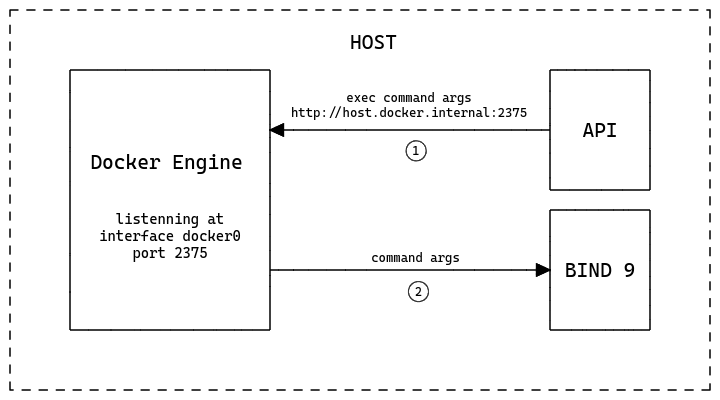
\includegraphics[width=\linewidth]{draws/extra_hosts.png}
    \caption{Ejecución de comandos desde el contenedor de la API al de BIND 9. En el paso 1, la API debe acceder al motor de Docker que maneja a BIND 9. Una vez recibido el pedido, el motor ejecuta el comando, paso 2, directamente en el contenedor de BIND 9.}
    \label{fig:extra_hosts}
\end{figure}

Para el servicio de BIND 9 fue usada la imagen que ofrece Ubuntu en DockerHub, ya mencionada en la sección \ref{sec:bind-storage}. La imagen de la API fue creada usando construcción de varias etapas (\textit{multi-stage build}) para minimizar considerablemente el tamaño de la imagen en producción [\cite{multi-stage}].

\begin{lstlisting}[frame=single, escapechar=|, caption=Dockerfile para la API.]
FROM docker.uclv.cu/golang:1.19.2 as base

ENV CGO_ENABLED=0

WORKDIR /go/src

COPY . .

RUN go build -mod=vendor -o build/bind-api
    

FROM scratch as prod|\label{line:2nd-stage}|

ENV GIN_MODE=release

COPY --from=base /go/src/build/bind-api /usr/bin/bind-api

VOLUME [ "/data/bind/conf", "/data/bind/lib", "/data/api" ]

EXPOSE 2020

CMD ["bind-api"]
\end{lstlisting}

En una primera etapa (\verb|base|) se usa como capa la imagen la imagen de Go, \verb|golang:1.19.2|, a ella se copian las dependencias del proyecto previamente creadas por \verb|go mod vendor|. Una vez hecho esto, es compilado el sistema en un único binario con todas sus dependencias autocontenidas.

La segunda etapa (línea \ref{line:2nd-stage}) tiene como objetivo crear una imagen con el número mínimo de artefactos. Esto se logra copiando tan solo el binario compilado del código fuente en la primera etapa. A continuación, con vistas a la puesta en producción, son especificados los volúmenes y el puerto a usar. En esta se usa como base la imagen \verb|scratch|\footnote{\url{https://hub.docker.com/_/scratch}}, una imagen especial de Docker, la cual no crea una capa extra al ser usada como punto de partida y que no contiene archivos.

Con el empleo de esta aproximación se logra disminuir considerablemente el tamaño de la imagen resultante. La primera etapa da como resultado una imagen de 1.15GB de tamaño, mientras que la segunda tan solo 19MB. Se reduce el tamaño final aproximadamente un 98.3\% al eliminar el SDK de Go y otras herramientas que trae la imagen por defecto. Estas no son necesarias en producción, dado que la aplicación es compilada en un solo archivo binario que se comunica directamente con el kernel de Linux.

\section{Experimentación}

Una vez concluida la propuesta y el desarrollo de su implementación, corresponde validar la solución creada. Para ello se modelan diferentes experimentos que verifiquen las funciones del servidor y su capacidad de respuesta. Con tal objetivo, se puede confirmar que la propuesta responde al problema para el que fue diseñada, pero además es posible verificar la carga a soportar de la implementación sobre BIND 9 y diferentes métricas que diagnostiquen la capacidad del servidor.

Primero, se trata de probar que añadir una nueva zona a través de la API, en efecto, modifica la configuración del servidor de nombres. Este experimento, además sirve para comprobar la latencia de la API al aumentar la cantidad de zonas que mantiene el servidor de BIND.

Segundo, se desea valorar el consumo de memoria por la API cuando el servidor maneja un número alto de zonas. Esto permite estimar la cantidad de zonas posibles a manejar de acuerdo a los recursos de cómputo.

Como tercera prueba, se realizan consultas DNS a BIND 9, de forma programática y manual para verificar que responde con la información requerida. Finalmente se muestran vistas de la interfaz web diseñadas que reflejan el uso de la API por esta para modificar la configuración de BIND 9.

Para la realización de los experimentos se usó la imagen de Docker usada en desarrollo y almacenada en el repositorio\footnote{\url{https://github.com/svex99/bind-api/blob/main/docks/dev.Dockerfile}}. Esta fue ejecutada en un ambiente con Ubuntu 22.04.1 LTS, procesador AMD Ryzen 5 5600h × 12, 8GB de RAM y 100GB de almacenamiento SSD.

\subsection{Latencia ante el aumento de la cantidad de zonas}

Para desarrollar este experimento el servidor fue poblado con una cantidad específica de zonas de forma previa. Cada fichero de zona creado tuvo un tamaño aproximado de 182B, lo que se traduce en una entrada en la configuración de BIND de aproximadamente 89B, y un total de 271B a procesar por cada zona. Cada una de las zonas solo tiene definidos tres registros, el \verb|SOA|, junto a un \verb|NS| y \verb|A| para indicar el servidor de nombres de la zonas. Esta información trae consigo un aumento de la carga en el servidor de BIND así como en la API, principalmente a la hora de ejecutar \verb|rndc reconfig| contra el servidor de nombres.

\begin{table}[!ht]
    \centering
    \begin{tabular}{|c|c|c|}
    \hline
    \multicolumn{1}{|p{4cm}|}{\centering\textbf{Zonas previas}} & \multicolumn{1}{|p{4cm}|}{\centering \textbf{Añadir 100 nuevas zonas (s)}} & \multicolumn{1}{|p{4cm}|}{\centering \textbf{Tiempo estimado por solicitud (ms)}} \\ \hline
        0 & 6.99 & 69.89 \\ \hline
        250 & 11.04 & 110.37 \\ \hline
        500 & 12.38 & 123.80 \\ \hline
        1000 & 14.15 & 141.51 \\ \hline
        2000 & 18.10 & 180.96 \\ \hline
        4000 & 24.66 & 246.55 \\ \hline
    \end{tabular}
    \caption{Tiempo de procesamiento de añadir 100 nuevas zonas de acuerdo al número de zonas previas.}
    \label{table:add-zones}
\end{table}

El tiempo necesario para dar respuesta ante un pedido es aceptable (tabla \ref{table:add-zones}), teniendo en cuenta la necesidad de comunicarse con el servidor de nombres. Este es el principal factor que aumenta el tiempo de respuesta, pues BIND 9 tiene que cargar cada una de las zonas en su configuración. El tiempo de respuesta aumenta a medida que toma más tiempo para el servidor procesar la solicitud de \verb|rdnc reconfig|. Además, la escritura en disco de la configuración cuando es añadida una nueva zona también aumenta, pues en sucesivas escrituras esta es reescrita.

La latencia de retribuir la lista completa de zonas, es baja (tabla \ref{table:get-zones}). La principal ventaja es que no se requiere de lectura en disco. La API mantiene una copia en memoria de la configuración del servidor de BIND con la cual responder a estos pedidos.

\begin{table}[!ht]
    \centering
    \begin{tabular}{|c|c|c|}
    \hline
    \multicolumn{1}{|p{4cm}|}{\centering\textbf{Zonas previas}} & \multicolumn{1}{|p{7cm}|}{\centering \textbf{Obtener la lista de zonas (ms)}} \\ \hline
        250  & 0.008740  \\ \hline
        500  & 0.019530  \\ \hline
        1000 & 0.056963  \\ \hline
        2000 & 0.174529  \\ \hline
        4000 & 0.182631  \\ \hline
    \end{tabular}
    \caption{Tiempo de procesamiento de obtener la lista de zonas de acuerdo al número de zonas previas.}
    \label{table:get-zones}
\end{table}

\subsection{Consumo de memoria ante el aumento de la cantidad de zonas}

Para medir el uso de memoria al cargar la información en memoria (invocar \verb|load|), se hizo uso de la biblioteca \verb|runtime/pprof|\footnote{\url{https://pkg.go.dev/runtime/pprof}} que viene por defecto en la instalación de Go. La herramienta del mismo nombre es usada para mostrar y analizar la información recogida en tiempo de ejecución. En este experimento se crearon zonas de forma semejante al anterior para desarrollar los pruebas.

\begin{figure}
    \centering
    \begin{subfigure}{0.49\textwidth}
        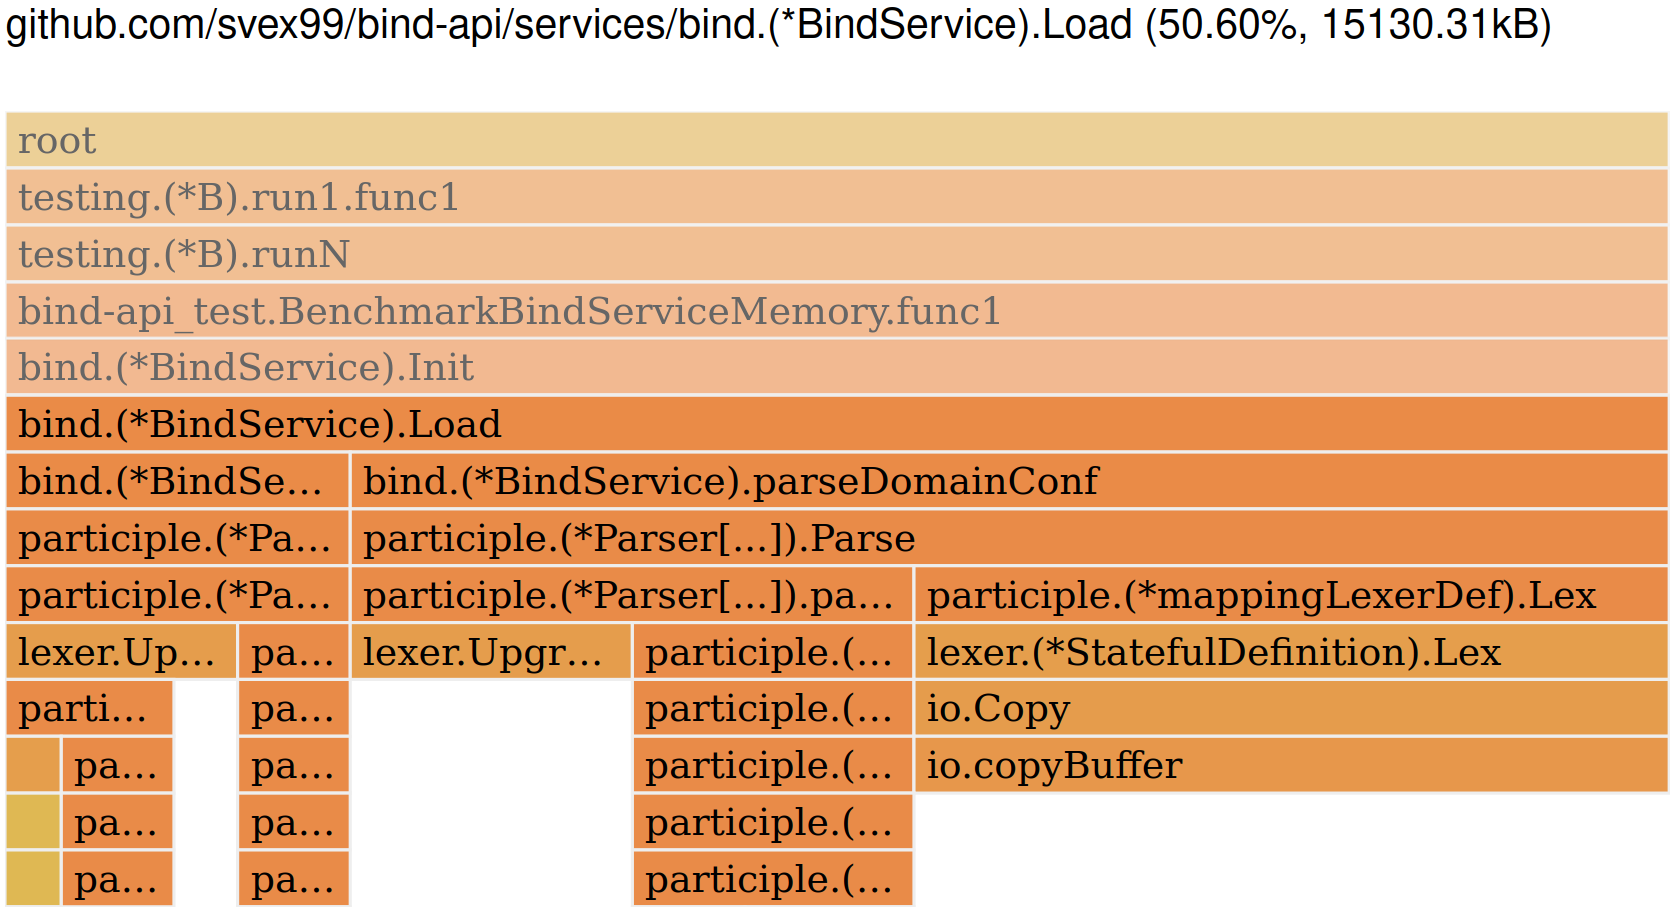
\includegraphics[width=\textwidth]{Graphics/mem250z.png}
        \caption{250 zonas}
    \end{subfigure}
    \hfill
    \begin{subfigure}{0.49\textwidth}
        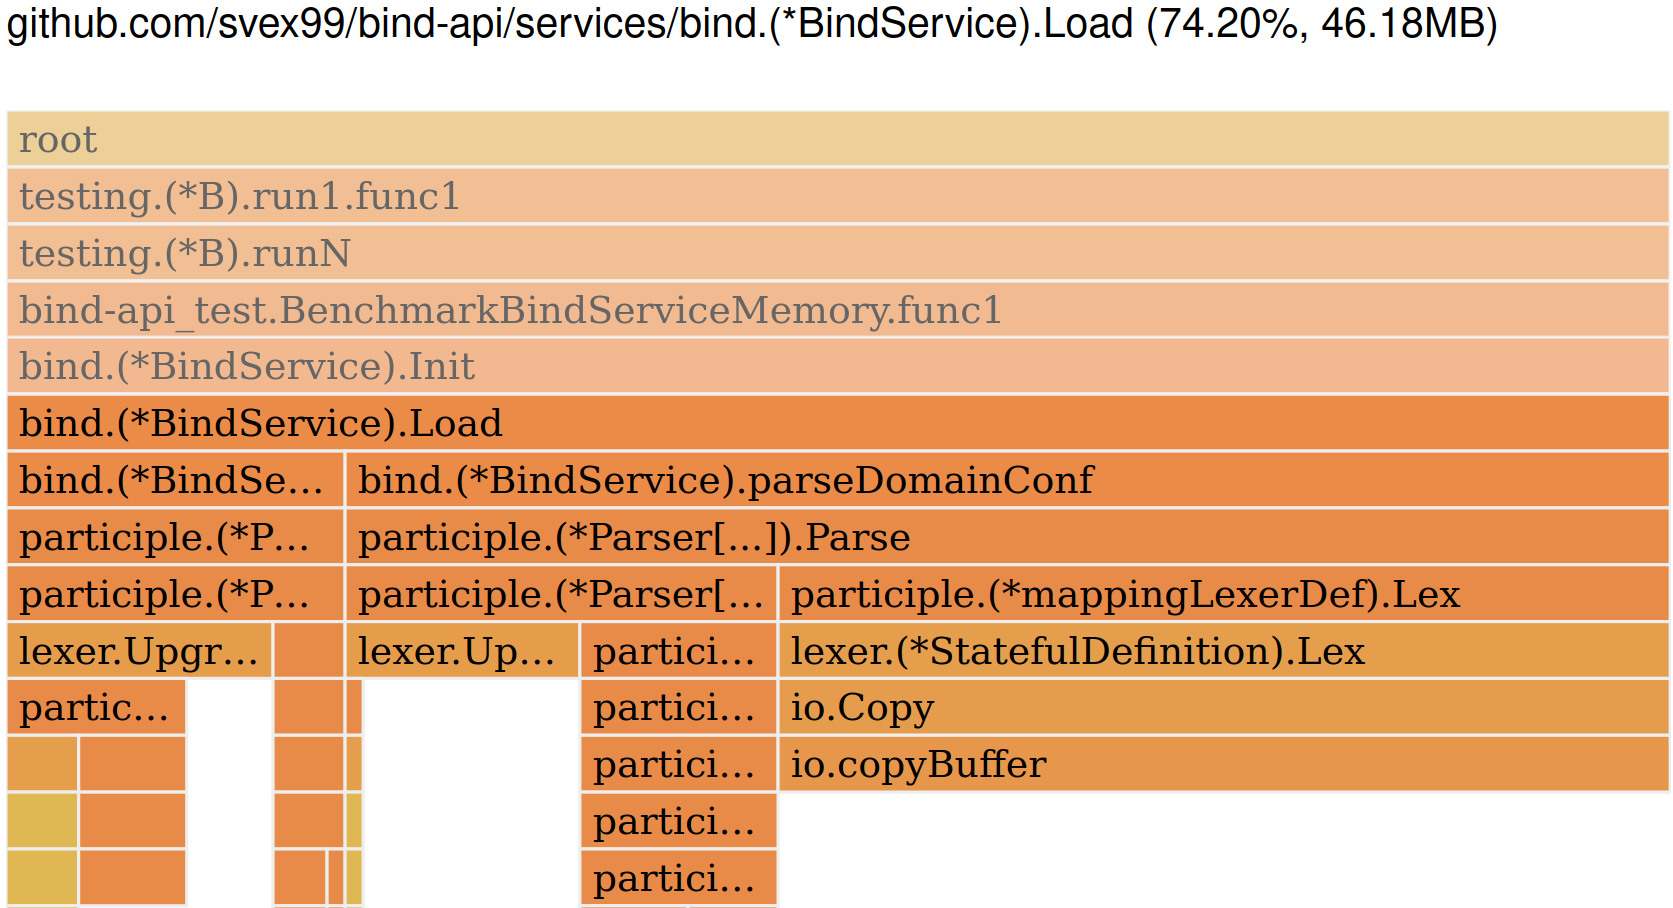
\includegraphics[width=\textwidth]{Graphics/mem500z.png}
        \caption{500 zonas}
    \end{subfigure}
    \hfill
    \begin{subfigure}{0.49\textwidth}
        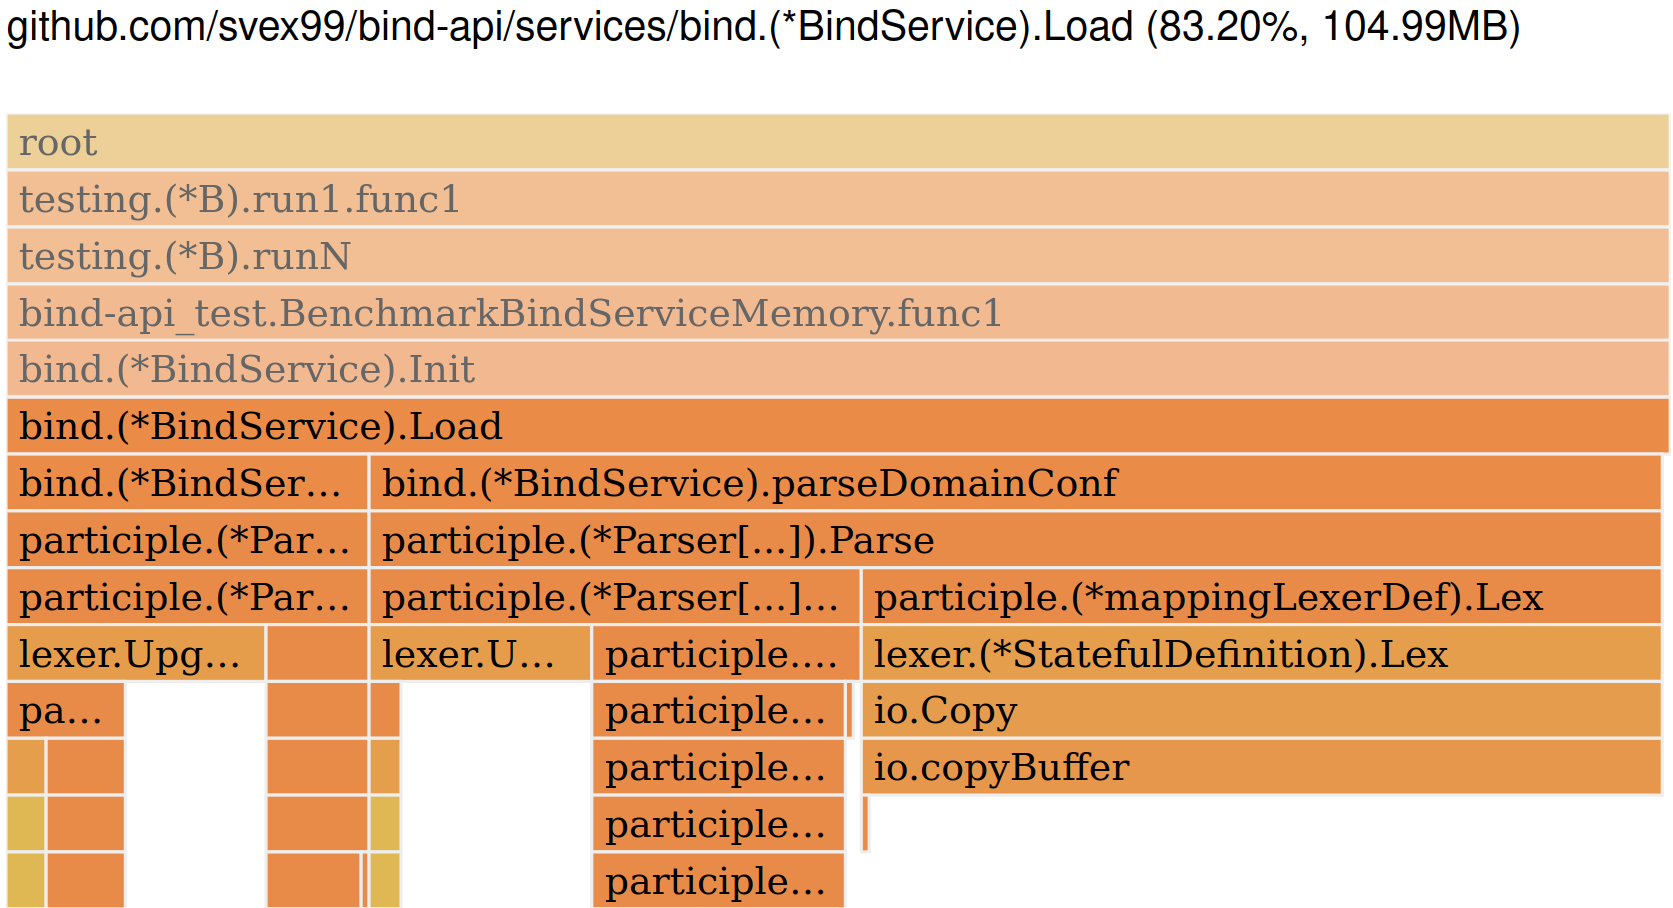
\includegraphics[width=\textwidth]{Graphics/mem1000z.png}
        \caption{1000 zonas}
    \end{subfigure}
    \hfill
    \begin{subfigure}{0.49\textwidth}
        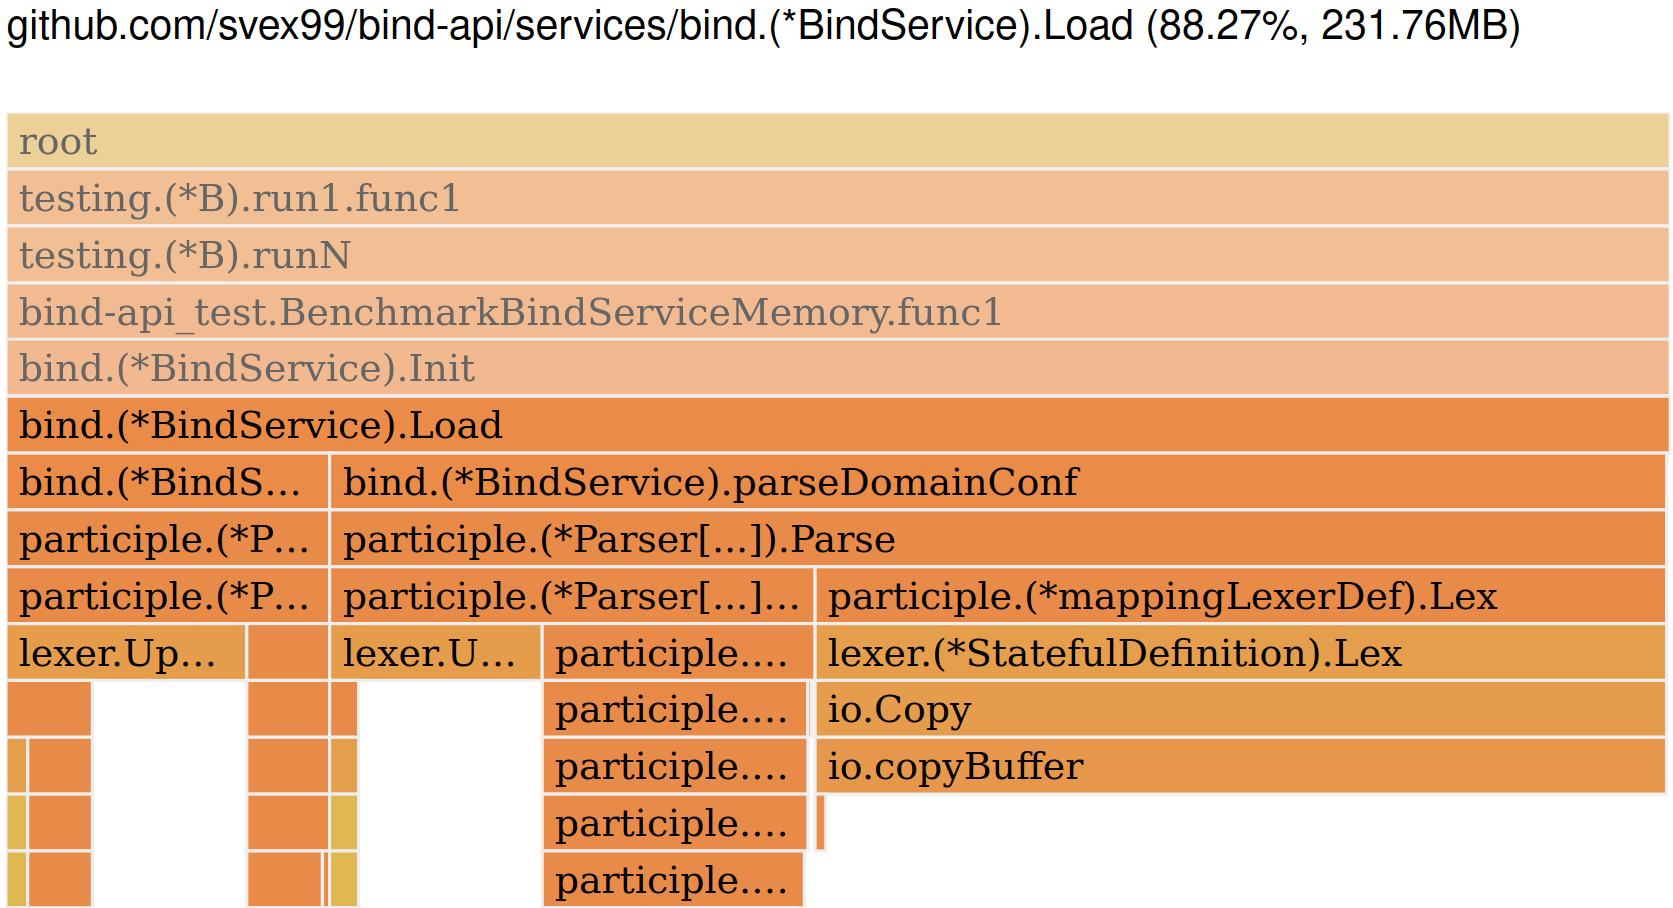
\includegraphics[width=\textwidth]{Graphics/mem2000z.png}
        \caption{2000 zonas}
    \end{subfigure}
    \hfill
    \begin{subfigure}{0.49\textwidth}
        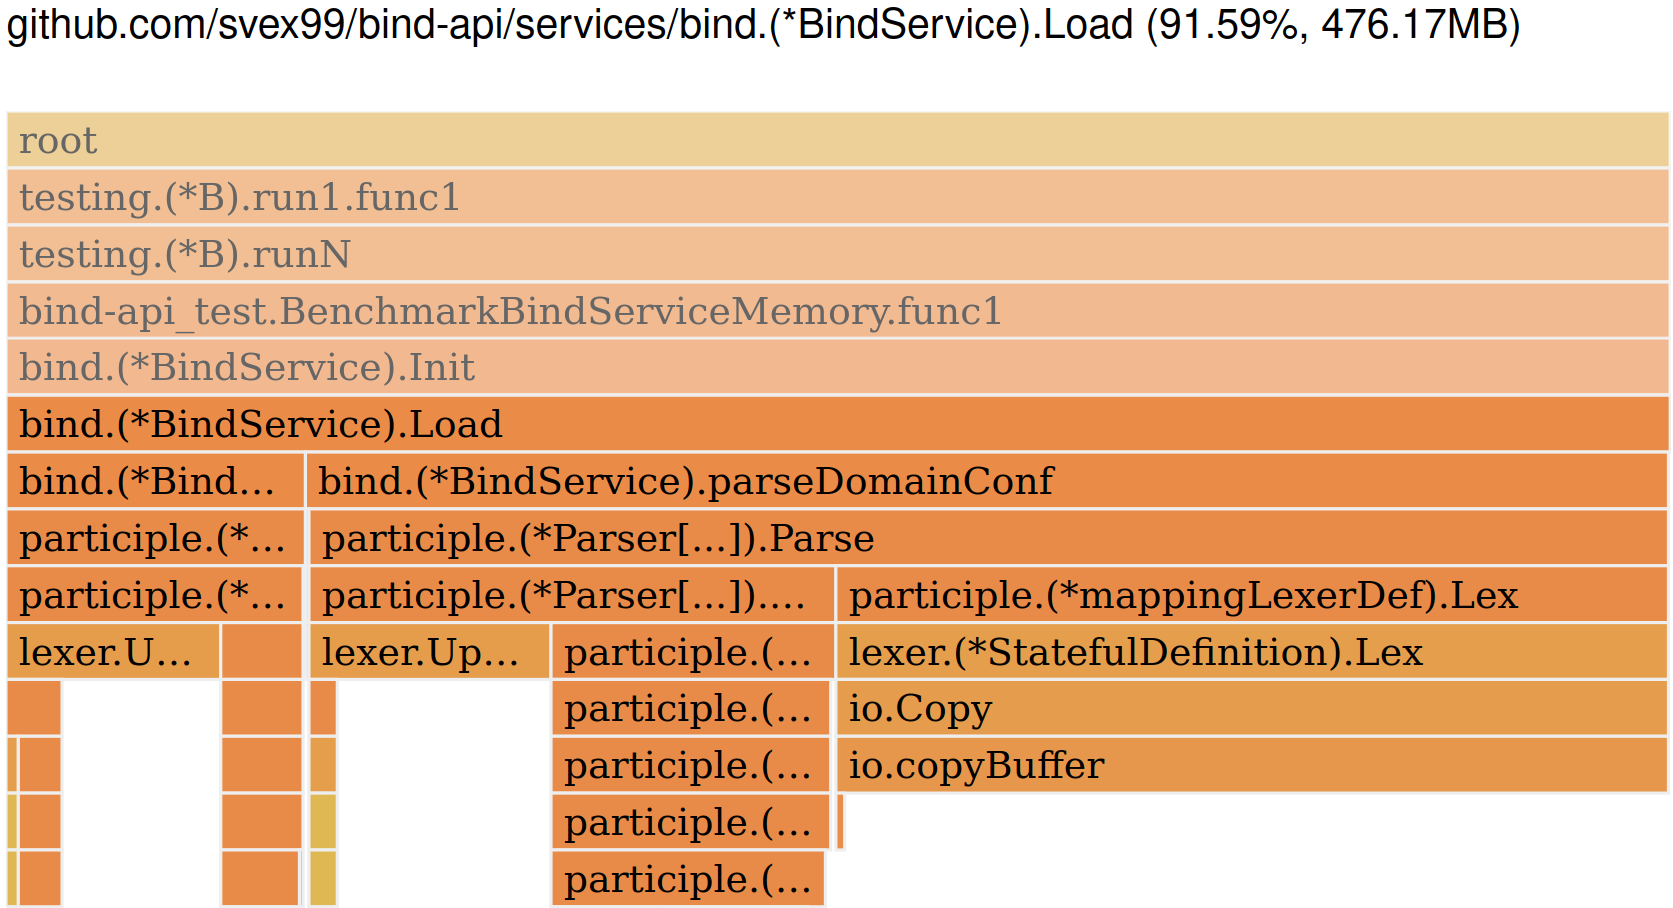
\includegraphics[width=\textwidth]{Graphics/mem4000z.png}
        \caption{4000 zonas}
    \end{subfigure}
    \hfill
    \begin{subfigure}{0.49\textwidth}
        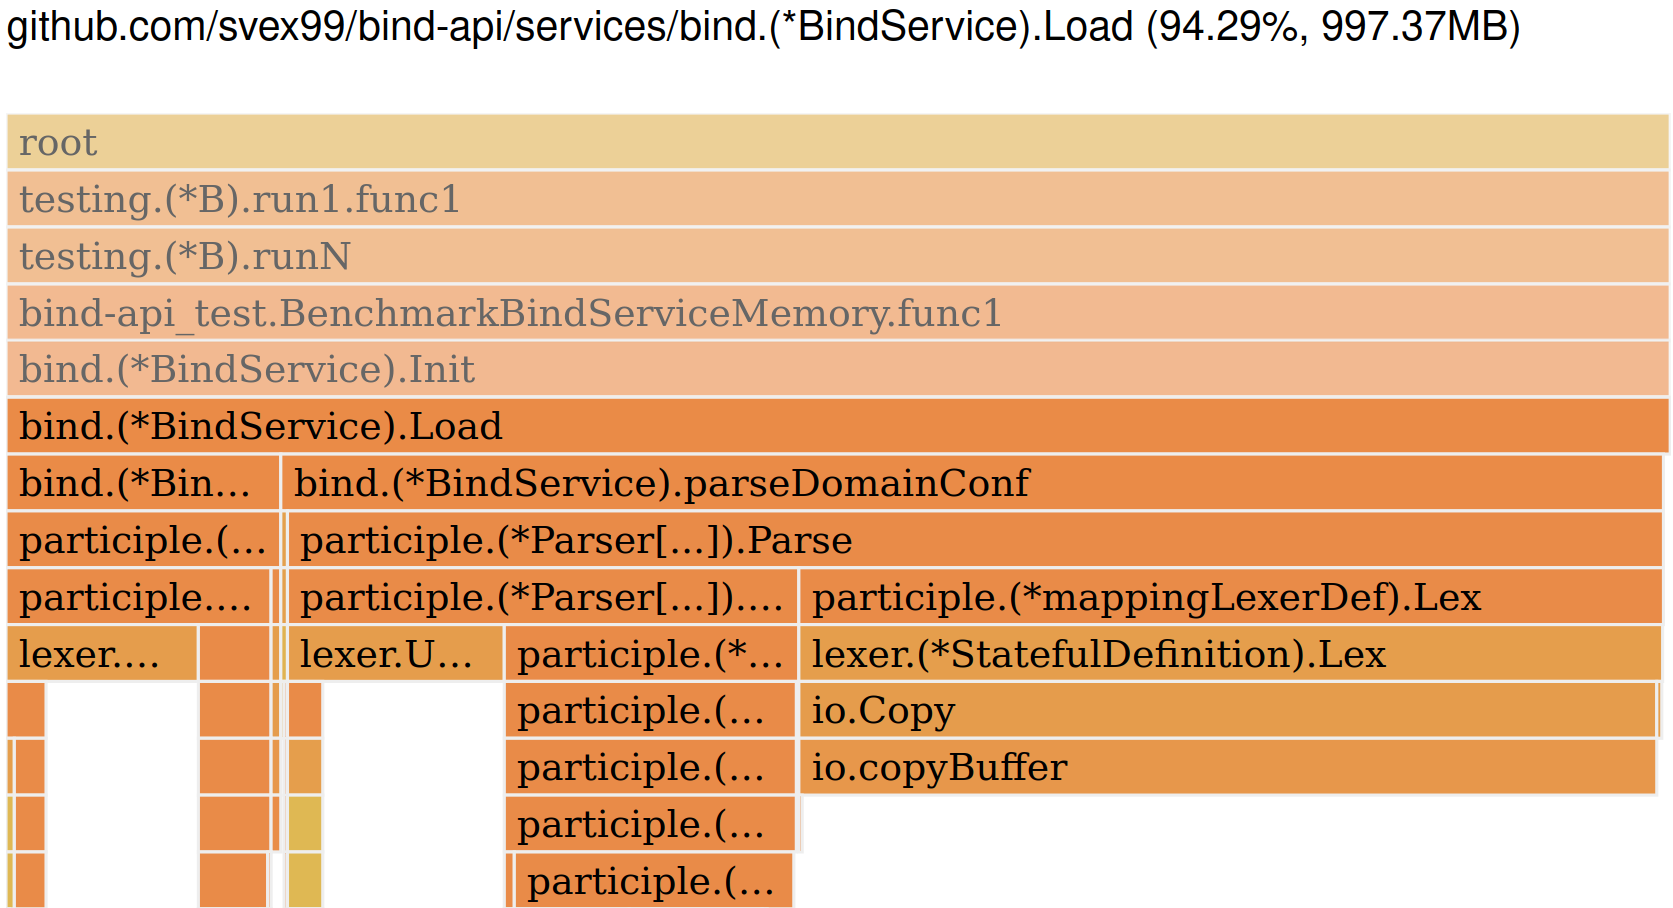
\includegraphics[width=\textwidth]{Graphics/mem8000z.png}
        \caption{8000 zonas}
    \end{subfigure}

    \caption{Consumo de memoria de la implementación de \textbf{load} de acuerdo a la cantidad de zonas.}
    \label{fig:bench-mem}
\end{figure}

Se puede apreciar en la figura \ref{fig:bench-mem} que la cantidad de zonas que maneje el servidor de nombres incurre directamente en el consumo de memoria de la API. El consumo inicial con 250 zonas es de apenas unos MB, llegando a consumir casi 1GB de RAM cuando maneja 8000 zonas, aproximadamente el 94\% de la memoria usada por el proceso.

El consumo de memoria también es directamente proporcional a la información almacenada en cada zona. Sin embargo, algunos proveedores recomiendan mantener la cantidad de zonas en un servidor DNS por debajo de 10000 [\cite{dns-cap}]. Por lo que ante un consumo de memoria elevado, la solución potencial puede ser escalar de forma horizontal con otro servicio, aunque también es necesario tener en cuenta la carga sobre el servidor.

\subsection{Pruebas End-to-End}

Estas pruebas está diseñadas con el objetivo de verificar que el servidor de BIND 9 manejado desde la API sirve la información de forma correcta. La configuración para desarrollar dicha prueba esta compuesta por BIND 9 y la API, ubicados en una red privada de Docker, con el primero sirviendo consultas DNS externas a través de un puerto expuesto para conexiones TCP y UDP. El contenedor de la API usa como servidor DNS a BIND 9 con el objetivo de realizar las consultas de prueba contra él.

En este ambiente se implementa un grupo de pruebas que, de forma programática, invocan los puntos finales de la API y consultan al servidor DNS para comprobar el correcto funcionamiento. Al ejecutar el conjunto de pruebas en el ambiente interno de Docker, las consultas DNS son resueltas de forma correcta con el servidor DNS. 

\begin{lstlisting}[frame=single, numbers=none, caption=Resultados del conjunto de pruebas \textit{end-to-end}.]
--- PASS: TestAPIFlow (8.73s)
    --- PASS: TestAPIFlow/TestAddZone (1.43s)
    --- PASS: TestAPIFlow/TestMXRecord (0.42s)
        --- PASS: TestAPIFlow/TestMXRecord/TestAddMX (0.34s)
        --- PASS: TestAPIFlow/TestMXRecord/TestDelMX (0.08s)
    --- PASS: TestAPIFlow/TestCNAMERecord (0.33s)
        --- PASS: TestAPIFlow/TestCNAMERecord/TestAddCNAME (0.26s)
        --- PASS: TestAPIFlow/TestCNAMERecord/TestDelCNAME (0.08s)
    --- PASS: TestAPIFlow/TestTXTRecord (0.43s)
        --- PASS: TestAPIFlow/TestTXTRecord/TestAddTXT (0.13s)
        --- PASS: TestAPIFlow/TestTXTRecord/TestDelTXT (0.30s)
    --- PASS: TestAPIFlow/TestDelZone (6.09s)
PASS
ok      github.com/svex99/bind-api      8.745s
\end{lstlisting}

Desde la computadora que realiza las pruebas y externo al ambiente de Docker, también es verificada esta información usando la herramienta \verb|dig|\footnote{\url{https://man.openbsd.org/dig.1}} para realizar consultas al servidor de nombres. A continuación, se toma como referencia un archivo de zona, y las consultas realizadas al servidor relacionadas con él.

\begin{lstlisting}[frame=single, numbers=none, caption=Archivo de registros para la zona \textbf{flow-test-1.com} servida por el servidor de BIND 9.]
$ORIGIN flow-test-1.com.
$TTL 2d
@ IN SOA ns1 svex ( 2022112514 86400 7200 3600000 172800 )
@ IN NS ns1
ns1 IN A 10.1.3.1
@ IN MX 101 email-server1
@ IN MX 103 email-server3
cname-dest IN A 7.7.7.7
@ IN TXT "key1=value-body"
\end{lstlisting}

\begin{lstlisting}[frame=single, numbers=none, caption=Consulta externas realizadas al servidor para la zona \textbf{flow-test-1.com}.]
$ dig +short @localhost -p 30053 flow-test-1.com soa
ns1.flow-test-1.com. svex.flow-test-1.com. 2022112514 86400 7200 3600000 172800

$ dig +short @localhost -p 30053 ns1.flow-test-1.com
10.1.3.1

$ dig +short @localhost -p 30053 flow-test-1.com mx 
101 email-server1.flow-test-1.com.
103 email-server3.flow-test-1.com.

$ dig +short @localhost -p 30053 flow-test-1.com txt 
"key1=value-body"
\end{lstlisting}

La capacidad del servidor DNS para responder a cada una de las consultas realizadas, tanto programáticas como manuales, valida el funcionamiento del flujo diseñado. Siendo así efectiva la solución para administrar el servidor de nombres de BIND 9.

\subsection{Funcionalidad de la Web}

La interfaz web hace uso de los diferentes puntos finales de la API para modificar el servidor de BIND 9. El CRUD de los diferentes objetos del servidor de nombres puede realizarse a través de esta interfaz sin necesidad de interactuar con la API directamente (Figura \ref{fig:web-view}).

\begin{figure}
    \centering
    \begin{subfigure}{0.49\textwidth}
        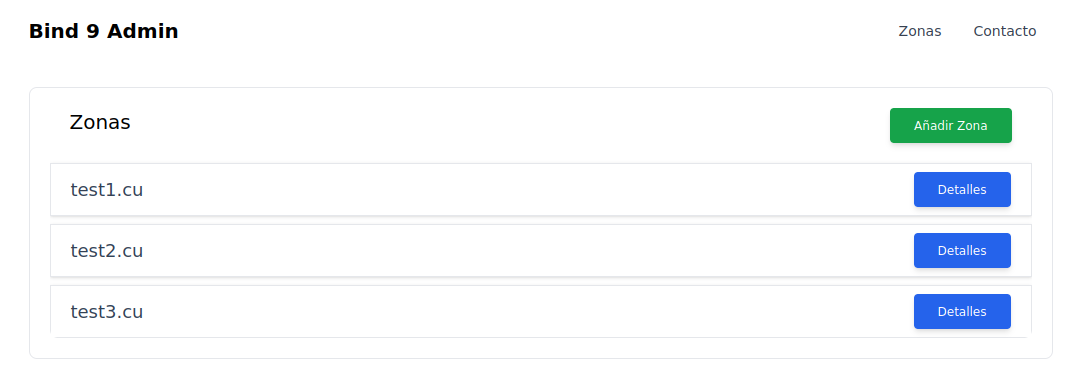
\includegraphics[width=\textwidth]{Graphics/web/list-zones.png}
        \caption{Vista para listar las diferentes zonas.}
    \end{subfigure}
    \hfill
    \begin{subfigure}{0.49\textwidth}
        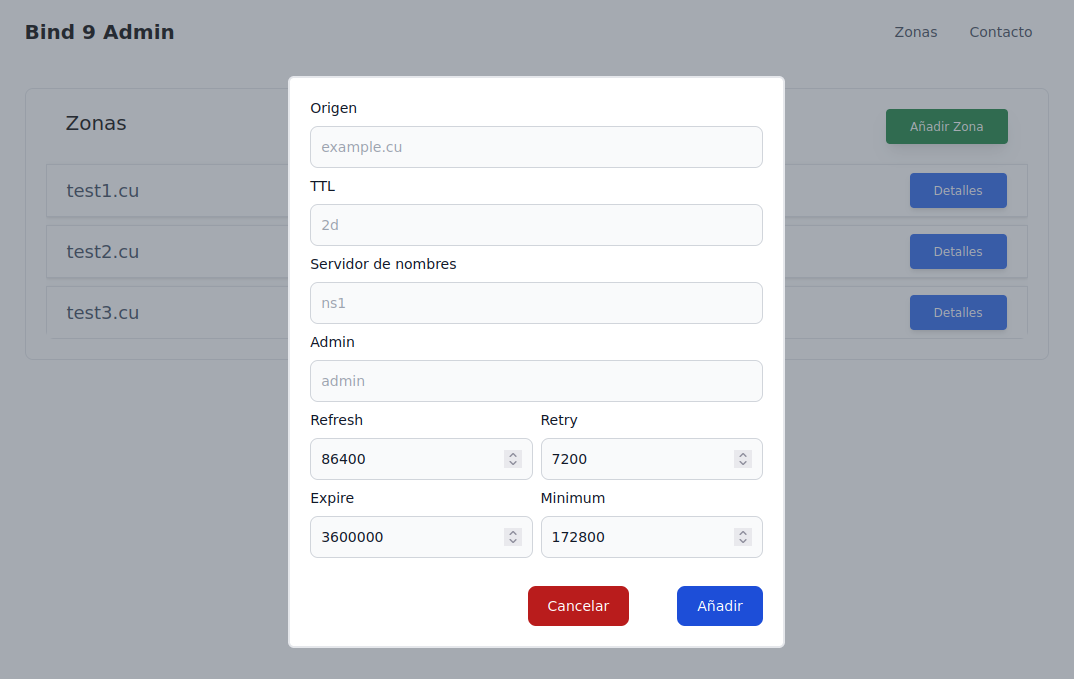
\includegraphics[width=\textwidth]{Graphics/web/add-zone.png}
        \caption{Formulario para añadir una nueva zona.}
    \end{subfigure}
    \hfill
    \begin{subfigure}{0.49\textwidth}
        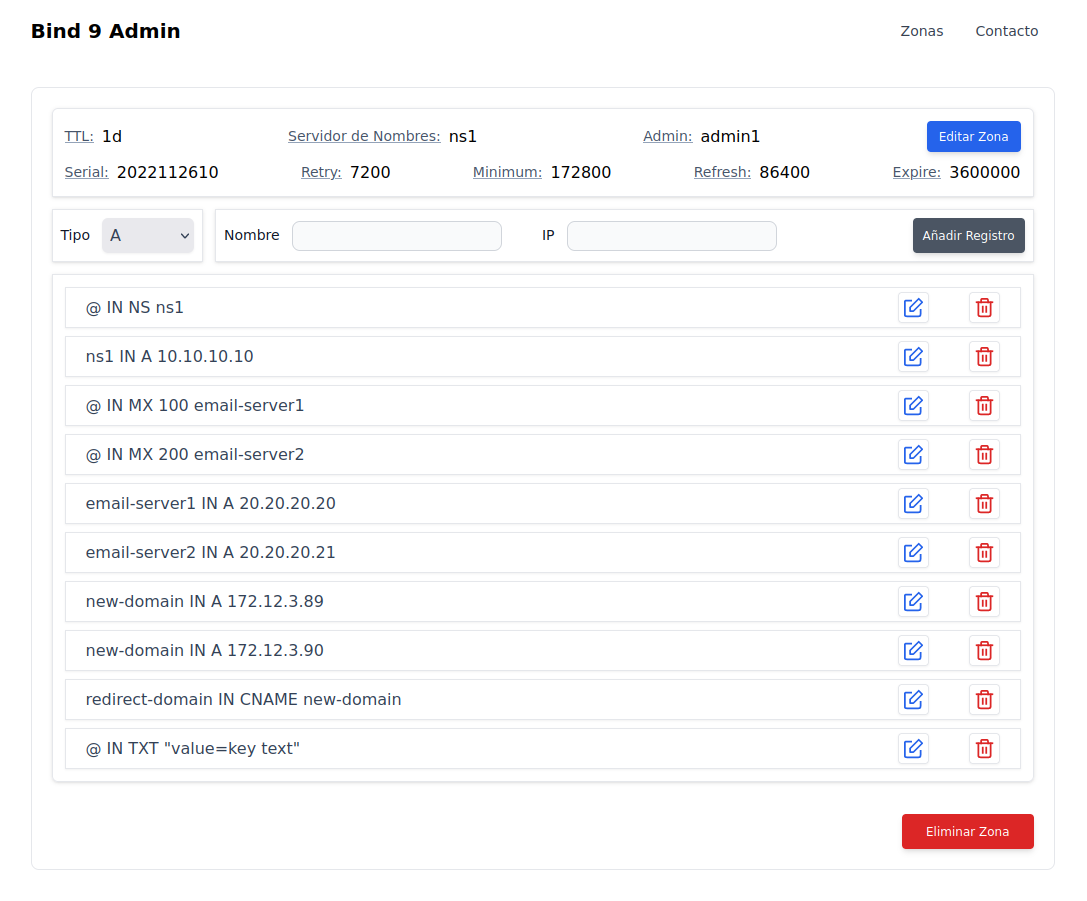
\includegraphics[width=\textwidth]{Graphics/web/list-records.png}
        \caption{Vista para administrar los detalles de una zona y los diferentes registros.}
    \end{subfigure}
    \hfill
    \begin{subfigure}{0.49\textwidth}
        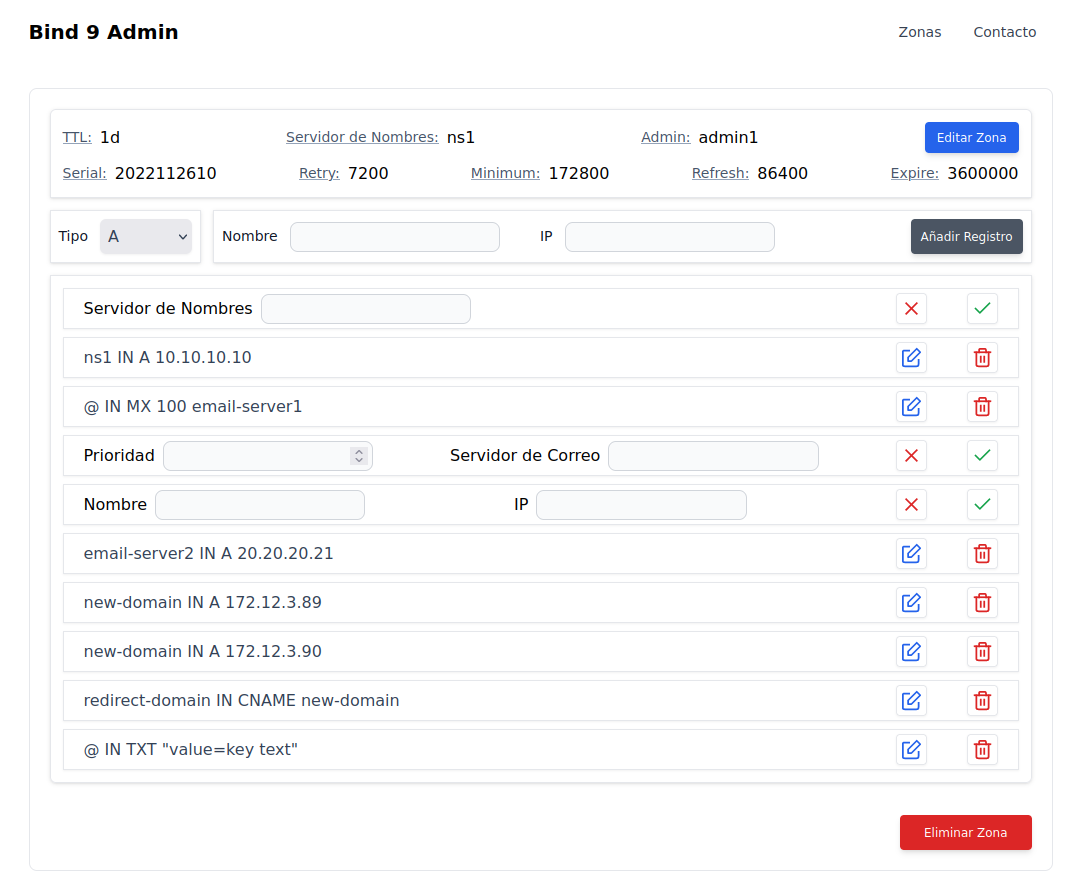
\includegraphics[width=\textwidth]{Graphics/web/edit-records.png}
        \caption{Opción para editar los registros.}
    \end{subfigure}

    \caption{Diferentes vistas de las página web.}
    \label{fig:web-view}
\end{figure}


\subsection{Discusión}

Los experimentos dan como resultado que la implementación de la propuesta es válida para su puesta en producción. Por tanto, un aproximación semejante en base a la propuesta puede aplicarse a otros servidores DNS autoritarios de código abierto. A pesar de esto, se considera que cada solución debe adaptarse a las cualidades del software al que aplica, como fue este caso con BIND 9.

En el entorno de la Universidad de La Habana, y organizaciones en general, las modificaciones ejecutadas sobre un servicio DNS a diario no llegan a ser altas para la capacidad de respuesta de la solución. Dado este caso, es válido aceptar como buenos los valores de latencia al hacer modificaciones sobre BIND y, por tanto, no es necesario considerar una optimización prematura sobre la misma.

El consumo de memoria es el principal aspecto a considerar a la hora de la puesta en producción, pero solo es acorde a la configuración que maneja el servidor de BIND. Positivamente, ofrece como ventaja obtener un tiempo de respuesta más rápido por parte de la API ante los pedidos.

La posibilidad de haber preparado la API para su despliegue con Docker permite limitar los recursos que esta usa a nivel de sistema. En el caso que la API y BIND 9 compartan recursos en una misma computadora y no sea posible estimarse el uso de memoria por la API, es posible desplegar el primero, limitando su uso de memoria, sin interferir con el funcionamiento del servicio DNS.

La interfaz web ofrece la facilidad de interactuar con la configuración del servidor de nombres y manejar tanto las zonas como el conjunto de registros que estas poseen. Cada una de las funciones derivadas de la función \verb|save| propuesta es usada indirectamente para responder a las modificaciones realizadas desde la interfaz web. Al ofrecer una aplicación de página simple la navegación es fluida una vez cargada la página inicial. Adicionalmente, el diseño es responsivo lo que permite la configuración desde un teléfono móvil o pantallas pequeñas.

\backmatter

\begin{conclusions}
Se analizó el estado del arte de las soluciones DNS actuales y diferentes tecnologías de desarrollo web. A partir de ello, se identificó que los servidores DNS de código abierto, en su mayoría, no disponen de una API HTTP que facilite de forma programática su configuración. Sin embargo, todos comparten aspectos comunes de acuerdo a la definición actual de DNS, lo que ofrece una vía para generalizar sobre ellos.

Se propuso una arquitectura basada en dos funciones, \verb|load| y \verb|save|, para gestionar el sistema de almacenamiento de los servidores DNS de código abierto. Dichas funciones tienen como objetivo cargar la configuración del servidor DNS y escribir cambios al disco, respectivamente. Estas se encuentran ubicada en un entorno más amplio, orientado a microservicios, que sienta las bases para la interacción entre la API HTTP, el sistema de almacenamiento del servidor DNS, y dicho servidor.

Se escogió a BIND 9 para desarrollar la implementación y los experimentos, como muestra de la funcionalidad de la propuesta teórica, y para aplicar la solución de forma práctica sobre el entorno de La Universidad de La Habana, dónde se usa dicho software como solución DNS. Se usó Go y Gin para la implementación de la API, un proceso de \textit{parsing} para la manipulación de la configuración DNS, Docker para el despliegue de los microservicios, y Vue.js para la implementación de la aplicación web.

Las pruebas realizadas comprobaron la validez de la propuesta teórica y la efectividad de la implementación sobre BIND 9. En este sentido se discutió y aprobó la factibilidad de aplicar el software al servicio DNS de la Universidad de La Habana. La interfaz web ofrece la posibilidad de realizar modificaciones de forma más simple sobre BIND 9, por personal no especializado en este, o con acceso directo a su sistema de archivos.
\end{conclusions}

\begin{recomendations}
El sistema implementado sobre BIND 9 no es capaz de cubrir la definición completa de DNS actual. Esta es demasiado extensa para tratarla en el tiempo dispuesto por esta tesis. Por tanto se recomienda extender los \textit{parsers} creados para los archivos de almacenamiento de BIND 9, tanto para los de configuración, como de zona. La extensión de estos junto con los puntos finales de la API para exponer nuevos registros de zona aumentaría la funcionalidad de la implementación.

Se propone, además, incorporar al sistema un \textit{driver} para volúmenes de Docker que permita ubicar la API en un motor de Docker distinto al que ser ubica el servidor DNS. El \textit{driver} permitiría ubicar el volumen que almacena la configuración del servidor DNS en un servicio externo y que tanto la API como BIND puedan acceder a él. Esto permitiría poder monitorear mejor los recursos para el servidor de BIND 9, y mantener este servicio crítico de forma aislada ante posibles vulnerabilidades en la API o insuficientes recursos para ambos bajo un mismo \textit{host}.

Adicionalmente, se propone implementar la propuesta sobre otros servidores de nombres autoritario de software libre. Documentar el proceso y realizar una comparación con la implementación desarrollada en esta tesis. 
\end{recomendations}

\include{BackMatter/Bibliography}

\end{document}